\documentclass[12pt]{article}
\usepackage{amsmath, esint}
\usepackage{amsthm}
\usepackage{amsfonts}
\usepackage{amssymb}
\usepackage{enumerate}
\usepackage{tikz}
\usepackage{tikz-cd}
\usepackage[margin = .75in]{geometry}
\usepackage[colorlinks=true, allcolors=purple]{hyperref}
\pagestyle{empty} 

\newcommand{\Nn}{\mathbb{N}} 
\newcommand{\Zz}{\mathbb{Z}} 
\newcommand{\Qq}{\mathbb{Q}}
\newcommand{\Rr}{\mathbb{R}}
\newcommand{\Cc}{\mathbb{C}}
\newcommand{\im}{\text{im}}
\newcommand{\m}{\mathfrak{m}}
\newcommand{\ann}{\text{ann}}
\newcommand{\ihat}{\hat{\textbf{i}}}
\newcommand{\jhat}{\hat{\textbf{j}}}
\newcommand{\khat}{\hat{\textbf{k}}}
\newcommand\set[1]{\{ #1 \}} %%\set{abc} ==> {abc}
\newcommand\abs[1]{\left| #1 \right|} %% \abs{abc} ==> |abc|
\newcommand\parens[1]{\left( #1 \right)} 
\newcommand\brac[1]{\left[ #1 \right]} 
\newenvironment{solution}
  {\renewcommand\qedsymbol{$\blacksquare$}\begin{proof}[Solution]}
  {\end{proof}}

% Dimensional tag. One of 1D, 1D in 2D, 1D in 3D, 2D, 2D in 3D, 3D.
\newcommand{\dimtag}[1]{{\footnotesize\textsc{[#1]}}\;}
% A short flow note set off from the problems. Intro sets the idea, story carries
% it on a running object, practice is the set below. No labels printed on those.
\newcommand{\flow}[1]{\par\noindent\textit{#1}\par\vspace{1mm}}


\begin{document}
\raggedright
\begin{center}
  {\large 2531 All questions}\\
  \vspace{5mm}
\end{center}


\section{Exam 1 Material}

\subsection{3D Coordinates and Geometry}

\subsubsection{Distance, Projections, and Spheres}
\begin{enumerate}
    \item \dimtag{2D in 3D} Only using the standard 2D Pythagorean theorem, find the distance from $(0,0,0)$ to $ (1,1,1)$.
    \item (Stewart \S12.1 \#14) Find the distance from the point $(4,-2,6)$ to each of the following. (a) the $xy$-plane, (b) the $yz$-plane, (c) the $xz$-plane, (d) the $x$-axis, (e) the $y$-axis, (f) the $z$-axis.
    \item (Stewart \S12.1 \#4) What are the projections of the point $(2, 3, 5)$ on the $xy$-, $yz$-, and $xz$-planes? Draw a rectangular box with the origin and $(2,3,5)$ as opposite vertices and with its faces parallel to the coordinate planes. Label all vertices of the box. Find the length of the diagonal of the box.
    \item (Stewart \S12.1 \#9) Find the distance between the points $(3,5,-2)$ and $(-1,1,-4)$.
    \item Find the equation of a sphere if one of its diameters has endpoints $(2, 1, 4)$ and $(4, 3, 10)$.
    \item (Stewart \S12.1 \#17) Find an equation of the sphere that passes through the point $(4,3,-1)$ and has center $(3,8,1)$.
    \item (Stewart \S12.1 \#16) Find an equation of the sphere with center $(2,-6,4)$ and radius $5$. Describe its intersection with each of the coordinate planes.
    \item (Stewart \S12.1 \#20) Show that the equation $x^2 + y^2 + z^2 = 6x - 4y - 10z$ represents a sphere, and find its center and radius.
    \item The figure shows a rectangular box with one vertex at the origin and the opposite vertex at $P$, with edges parallel to the coordinate axes.
    \begin{center}
    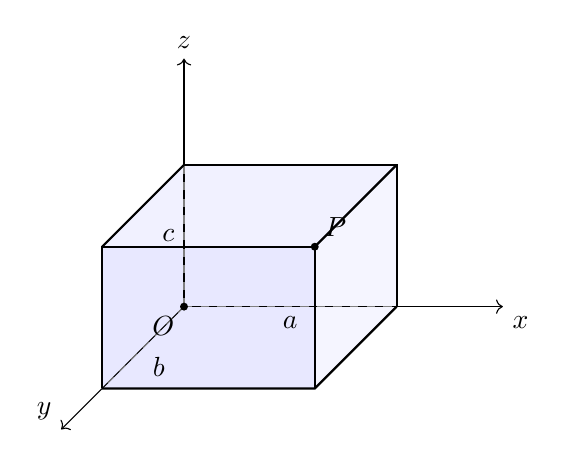
\begin{tikzpicture}[scale=0.9]
        \fill[blue!10,opacity=0.55] (0,2,0) -- (3,2,0) -- (3,2,3) -- (0,2,3) -- cycle;
        \fill[blue!16,opacity=0.55] (0,0,3) -- (3,0,3) -- (3,2,3) -- (0,2,3) -- cycle;
        \fill[blue!7,opacity=0.55]  (3,0,0) -- (3,2,0) -- (3,2,3) -- (3,0,3) -- cycle;
        \draw[->] (0,0,0) -- (4.5,0,0) node[below right]{$x$};
        \draw[->] (0,0,0) -- (0,3.5,0) node[above]{$z$};
        \draw[->] (0,0,0) -- (0,0,4.5) node[above left]{$y$};
        \draw[dashed,gray] (0,0,0) -- (3,0,0);
        \draw[dashed,gray] (0,0,0) -- (0,2,0);
        \draw[dashed,gray] (0,0,0) -- (0,0,3);
        \draw[thick] (3,0,0) -- (3,2,0) -- (0,2,0);
        \draw[thick] (3,0,0) -- (3,0,3) -- (0,0,3);
        \draw[thick] (0,2,0) -- (0,2,3);
        \draw[thick] (0,0,3) -- (0,2,3) -- (3,2,3) -- (3,0,3);
        \draw[thick] (3,2,0) -- (3,2,3);
        \fill (3,2,3) circle (1.6pt) node[above right]{$P$};
        \fill (0,0,0) circle (1.6pt) node[below left]{$O$};
        \node[below] at (1.5,0,0) {$a$};
        \node[left] at (0,1,0) {$c$};
        \node[below right] at (0,0,1.5) {$b$};
    \end{tikzpicture}
    \end{center}
    If $|OP| = 7$ and the edges along the $x$- and $y$-axes have lengths $a=3$ and $b=6$ respectively, find $c$ and the coordinates of $P$. Then find the lengths of all four space diagonals of the box.
    \item Find the midpoint of the segment joining $(1,3,-2)$ and $(5,-1,4)$.
    \item Find an equation of the sphere with center $(1,-4,3)$ and radius $5$, and decide whether $(3,-2,2)$ lies inside, on, or outside it.
    \item Show that $x^2+y^2+z^2+4x-6y+2z+5=0$ is a sphere by completing the square, and give its center and radius.
    \item Find the radius of the circle in which the sphere $x^2+y^2+z^2=9$ meets the plane $z=1$.
\end{enumerate}

\subsubsection{Octants, Regions, and Inequalities}
\begin{enumerate}
    \item \dimtag{3D} For what octants is $z\tan(y/x)$ positive or negative?
    \item (Stewart \S12.1 \#36) Sketch the region defined by $x^2 + z^2 \leq 25,\ 0 \leq y \leq 2$.
    \item Draw the region defined by the inequalities $x^2+z^2 \leq 25$ and $0 \leq y \leq 5$.
    \item (Stewart \S12.1 \#27--42) Describe in words the region of $\mathbb{R}^3$ represented by each equation.
    \begin{enumerate}
        \item $z = -2$ \quad (\#27)
        \item $y \geq 1$ \quad (\#29)
        \item $z = y$ \quad (\#32)
        \item $x^2 + y^2 = 4,\ z = -1$ \quad (\#33)
        \item $x^2 + y^2 + z^2 = 4$ \quad (\#37)
        \item $x^2 + y^2 + z^2 \leq 4$ \quad (\#38)
        \item $1 \leq x^2 + y^2 \leq 5$ \quad (\#40)
        \item $0 \leq x \leq 3,\ 0 \leq y \leq 3,\ 0 \leq z \leq 3$ \quad (\#41)
        \item $x^2 + y^2 + z^2 > 2z$ \quad (\#42)
    \end{enumerate}
    \item (Stewart \S12.1 \#43) Write inequalities to describe the region between the $yz$-plane and the vertical plane $x = 5$.
    \item (Stewart \S12.1 \#44) Write inequalities to describe the solid cylinder that lies on or below the plane $z=8$ and on or above the disk in the $xy$-plane with center the origin and radius $2$.
    \item Sketch the plane given by the equation $2x + 3y + z = 6$ in the first octant. Label the $x, y,$ and $z$ intercepts.
    \item A solid is bounded below by the disk $x^2+y^2\le 4$ in the $xy$-plane and above by the slanted plane $z = 4 - x$. The two figures below show the side view (cut by the $xz$-plane) and the top view.
    \begin{center}
    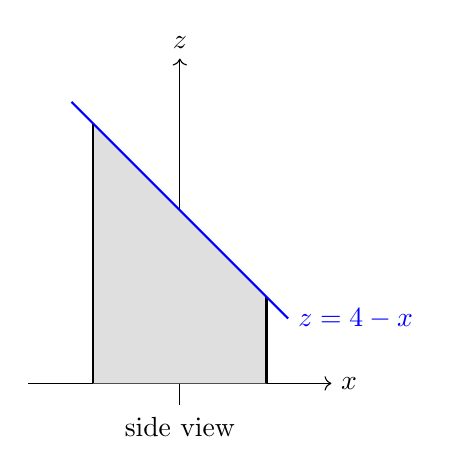
\begin{tikzpicture}[scale=0.55]
        \draw[->] (-3.5,0) -- (3.5,0) node[right]{$x$};
        \draw[->] (0,-0.5) -- (0,7.5) node[above]{$z$};
        \fill[gray!25] (-2,0) -- (-2,6) -- (2,2) -- (2,0) -- cycle;
        \draw[thick] (-2,0) -- (-2,6);
        \draw[thick] (2,0) -- (2,2);
        \draw[thick,blue] (-2.5,6.5) -- (2.5,1.5) node[right]{$z=4-x$};
        \node at (0,-1) {side view};
    \end{tikzpicture}\hspace{1.2cm}%
    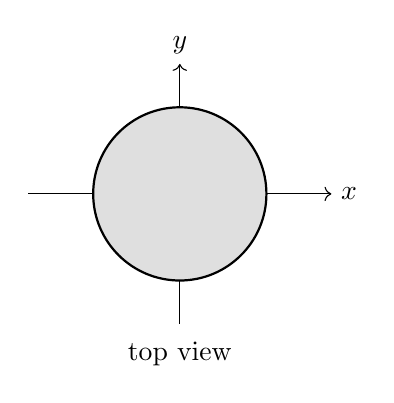
\begin{tikzpicture}[scale=0.55]
        \draw[->] (-3.5,0) -- (3.5,0) node[right]{$x$};
        \draw[->] (0,-3) -- (0,3) node[above]{$y$};
        \fill[gray!25] (0,0) circle (2);
        \draw[thick] (0,0) circle (2);
        \node at (0,-3.7) {top view};
    \end{tikzpicture}
    \end{center}
    Write a system of inequalities describing this solid, and find the largest and smallest $z$-values that occur in it.
    \item Describe in words the solid region $1\le x^2+y^2+z^2\le 4$, and sketch it.
    \item Write inequalities for the solid cylinder of radius $3$ about the $z$-axis lying between $z=0$ and $z=5$.
    \item Sketch the region $x^2+y^2\le z\le 4$ and describe its bounding surfaces.
\end{enumerate}

\subsection{Vectors}

\subsubsection{Vector Pictures and Basics}
\begin{enumerate}
    \item \dimtag{1D in 2D} Find a vector parallel to the line $y=2x+1$.
    \item Parameterize the line $y = 2x - 1$ as a directed curve $\vec{r}(t) = \langle x(t), y(t) \rangle$. Sketch the curve and mark the positions $\vec{r}(0)$ and $\vec{r}(1)$ with arrows indicating the direction of motion.
    \item A 2D vector has magnitude 2 and has an angle of $\pi/4$ with the positive $x$-axis. Express the vector in $a \ihat + b \jhat$ form. Also find a unit vector in the same direction.
    \item (Stewart \S12.2 \#27) What is the angle between the vector $\ihat + \sqrt{3}\,\jhat$ and the positive direction of the $x$-axis?
    \item (Stewart \S12.2 \#29) The initial point of a vector $\vec{v}$ in $V_2$ is the origin and the terminal point is in quadrant II. If $\vec{v}$ makes an angle $5\pi/6$ with the positive $x$-axis and $|\vec{v}| = 4$, find $\vec{v}$ in component form.
    \item (Stewart \S12.2 \#30) A child pulls a sled through the snow on a level path with a force of $50$ N exerted at an angle of $38^\circ$ above the horizontal. Find the horizontal and vertical components of the force.
    \item (Stewart \S12.2 \#9) Find a vector $\vec{a}$ with representation given by the directed line segment $\overrightarrow{AB}$, where $A(-2,1),\ B(1,2)$. Draw $\overrightarrow{AB}$ and the equivalent representation starting at the origin.
    \item (Stewart \S12.2 \#19) Let $\vec{a}=\langle -3,4\rangle$ and $\vec{b}=\langle 9,-1\rangle$. Find $\vec{a}+\vec{b}$, $4\vec{a}+2\vec{b}$, $|\vec{a}|$, and $|\vec{a}-\vec{b}|$.
    \item (Stewart \S12.2 \#24) Find a unit vector that has the same direction as $-5\ihat + 3\jhat - \khat$.
    \item Find the unit vector that is in the same direction as the vector from $P(1, 2, 3)$ to $Q(4, 6, 3)$.
    \item Let $O$ denote the origin of $\mathbb{R}^n$ and let $A,B \in \mathbb{R}^n$ be points. Let $C$ be the point on segment $AB$ that is twice as close to $A$ as to $B$ (that is, $|AC| = \tfrac{1}{2}|CB|$). Show that $\vec{OC} = \tfrac{2}{3}\vec{OA} + \tfrac{1}{3}\vec{OB}$.
    \item (Stewart \S12.2 \#44) Let $C$ be the point on the line segment $AB$ that is twice as far from $B$ as it is from $A$. If $\vec{a}=\overrightarrow{OA}$, $\vec{b}=\overrightarrow{OB}$, $\vec{c}=\overrightarrow{OC}$, show that $\vec{c} = \tfrac{2}{3}\vec{a} + \tfrac{1}{3}\vec{b}$.
    \item (Stewart \S12.2 \#43) If $A,B,C$ are the vertices of a triangle, find $\overrightarrow{AB} + \overrightarrow{BC} + \overrightarrow{CA}$.
    \item (Stewart \S12.2 \#41) Find the unit vectors that are parallel to the tangent line to the parabola $y = x^2$ at the point $(2,4)$.

    \item (Stewart \S12.2 \#3) Name all the equal vectors in the parallelogram shown.
    \begin{center}
    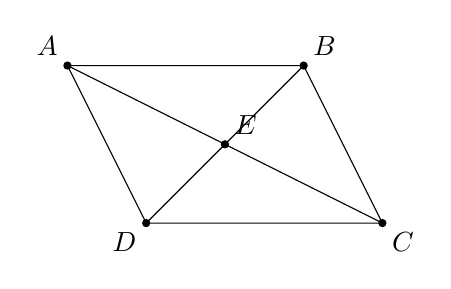
\begin{tikzpicture}[scale=1]
        \coordinate (A) at (0,2); \coordinate (B) at (3,2);
        \coordinate (D) at (1,0); \coordinate (C) at (4,0);
        \coordinate (E) at (2,1);
        \draw (A) -- (B) -- (C) -- (D) -- cycle;
        \draw (A) -- (C); \draw (B) -- (D);
        \foreach \p/\pos in {A/above left, B/above right, C/below right, D/below left, E/above right}
            \fill (\p) circle (1.5pt) node[\pos]{$\p$};
    \end{tikzpicture}
    \end{center}

    \item (Stewart \S12.2 \#4) Using the vectors in the figure, write each sum or difference as a single vector.
    (a) $\overrightarrow{AB} + \overrightarrow{BC}$,\quad
    (b) $\overrightarrow{CD} + \overrightarrow{DB}$,\quad
    (c) $\overrightarrow{DB} - \overrightarrow{AB}$,\quad
    (d) $\overrightarrow{DC} + \overrightarrow{CA} + \overrightarrow{AB}$.
    \begin{center}
    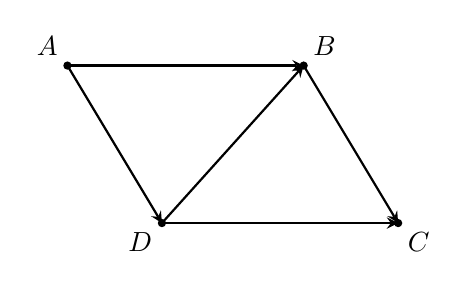
\begin{tikzpicture}[scale=1, >=stealth]
        \coordinate (A) at (0,2);   \coordinate (B) at (3,2);
        \coordinate (D) at (1.2,0); \coordinate (C) at (4.2,0);
        \draw[->,thick] (A)--(B); \draw[->,thick] (B)--(C);
        \draw[->,thick] (D)--(C); \draw[->,thick] (A)--(D); \draw[->,thick] (D)--(B);
        \foreach \p/\pos in {A/above left, B/above right, C/below right, D/below left}
            \fill (\p) circle (1.5pt) node[\pos]{$\p$};
    \end{tikzpicture}
    \end{center}

    \item (Stewart \S12.2 \#6) Using the vectors $\vec{u}$ and $\vec{v}$ in the figure, sketch each of these.
    (a) $\vec{u}+\vec{v}$,\ (b) $\vec{u}-\vec{v}$,\ (c) $2\vec{u}$,\ (d) $-\tfrac12 \vec{v}$,\ (e) $3\vec{u}+\vec{v}$,\ (f) $\vec{v}-2\vec{u}$.
    \begin{center}
    \begin{tikzpicture}[scale=1, >=stealth]
        \draw[->,thick] (0,0) -- (1.5,0.8) node[midway,above]{$\vec{u}$};
        \draw[->,thick] (3,0) -- (4.5,-0.6) node[midway,below]{$\vec{v}$};
    \end{tikzpicture}
    \end{center}

    \item (Stewart \S12.2 \#8) If the vectors in the figure satisfy $|\vec{u}|=|\vec{v}|=1$ and $\vec{u}+\vec{v}+\vec{w}=\vec{0}$, what is $|\vec{w}|$?
    \begin{center}
    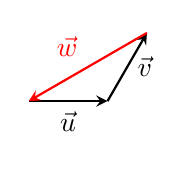
\begin{tikzpicture}[scale=1, >=stealth]
        \draw[->,thick] (0,0) -- (1,0) node[midway,below]{$\vec{u}$};
        \draw[->,thick] (1,0) -- (1.5,0.866) node[midway,right]{$\vec{v}$};
        \draw[->,thick,red] (1.5,0.866) -- (0,0) node[midway,above left]{$\vec{w}$};
    \end{tikzpicture}
    \end{center}

    \item (Stewart \S12.2 \#32) Find the magnitude of the resultant force and the angle it makes with the positive $x$-axis.
    \begin{center}
    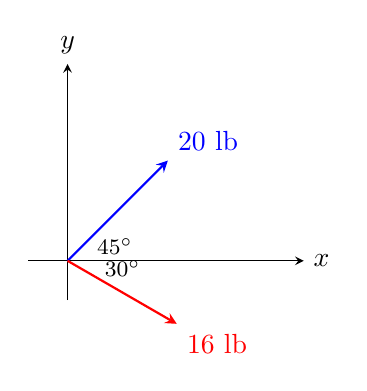
\begin{tikzpicture}[scale=1, >=stealth]
        \draw[->] (-0.5,0) -- (3,0) node[right]{$x$};
        \draw[->] (0,-0.5) -- (0,2.5) node[above]{$y$};
        \draw[->,thick,blue] (0,0) -- ({1.8*cos(45)},{1.8*sin(45)}) node[above right]{$20$ lb};
        \draw[->,thick,red]  (0,0) -- ({1.6*cos(-30)},{1.6*sin(-30)}) node[below right]{$16$ lb};
        \node at (0.6,0.18) {\footnotesize $45^\circ$};
        \node at (0.7,-0.1) {\footnotesize $30^\circ$};
    \end{tikzpicture}
    \end{center}

    \item (Stewart \S12.2 \#45) Let $\vec{a}=\langle 3,2\rangle$, $\vec{b}=\langle 2,-1\rangle$, $\vec{c}=\langle 7,1\rangle$.
    (a) Draw $\vec{a},\vec{b},\vec{c}$.
    (b) Show by a sketch that there are scalars $s$ and $t$ such that $\vec{c} = s\vec{a} + t\vec{b}$.
    (c) Use the sketch to estimate $s$ and $t$.
    (d) Find the exact values of $s$ and $t$.
    \item Find $|\vec a|$ and a unit vector in the direction of $\vec a=\langle 2,-3,6\rangle$.
    \item Find the vector from $P(1,2,-1)$ to $Q(4,-2,3)$ and its length.
    \item Find a vector of magnitude $10$ in the direction of $\langle 3,0,-4\rangle$.
    \item For $\vec a=\langle 1,2\rangle$ and $\vec b=\langle -3,1\rangle$, compute $2\vec a-3\vec b$ and $|\vec a+\vec b|$.
\end{enumerate}

\subsubsection{Dot Products and Projections}
\begin{enumerate}
    \item \dimtag{1D in 2D} If $\vec{a}= \langle 1,1 \rangle$ and $\vec{b}= \langle -1,2 \rangle$, draw a picture of and calculate $\text{orth}_{\vec{a}} \vec{b}$ and $\text{proj}_{\vec{a}}\vec{b}$.
    \item Find the angle $\theta$ between the vectors $\vec{u} = \langle 1, \sqrt{3} \rangle$ and $\vec{v} = \langle 1, 0 \rangle$.
    \item Find the angle $\theta$ between the vectors $\vec a = \langle 2, -1, 1 \rangle$ and $\mathbf{b} = \langle 1, 1, 2 \rangle$.
    \item Determine if the vectors $\vec{u} = \langle 2, 6, -4 \rangle$ and $\vec{v} = \langle -3, 1, 0 \rangle$ are orthogonal, parallel, or neither.
    \item (Stewart \S12.3 \#45) Show that $\text{orth}_{\vec{a}}\vec{b} = \vec{b} - \text{proj}_{\vec{a}}\vec{b}$ is orthogonal to $\vec{a}$ (this is why it is called the \emph{orthogonal projection} of $\vec{b}$).
    \item (Stewart \S12.3 \#46) For the vectors $\vec{a}=\langle 1,4\rangle$, $\vec{b}=\langle 2,3\rangle$, find $\text{orth}_{\vec{a}}\vec{b}$ and illustrate by drawing $\vec{a}, \vec{b}, \text{proj}_{\vec{a}}\vec{b}, \text{orth}_{\vec{a}}\vec{b}$.
    \item (Stewart \S12.3 \#63) \textbf{Parallelogram Identity.} The parallelogram identity states that
    \[ |\vec{a}+\vec{b}|^2 + |\vec{a}-\vec{b}|^2 = 2|\vec{a}|^2 + 2|\vec{b}|^2. \]
    (a) Give a geometric interpretation. (b) Prove the identity using the fact $|\vec{x}|^2 = \vec{x}\cdot\vec{x}$.
    \item In the figure, $|\vec{a}|=4$ and $|\vec{b}|=3$, and the angle between them is $\theta=60^\circ$.
    \begin{center}
    \begin{tikzpicture}[scale=1, >=stealth]
        \draw[->,thick] (0,0) -- (4,0) node[midway,below]{$\vec{a}$};
        \draw[->,thick] (0,0) -- ({3*cos(60)},{3*sin(60)}) node[above left]{$\vec{b}$};
        \draw (0.7,0) arc[start angle=0, end angle=60, radius=0.7];
        \node at (1.0,0.3) {\footnotesize $\theta$};
    \end{tikzpicture}
    \end{center}
    Compute $\vec{a}\cdot\vec{b}$, $\text{proj}_{\vec{a}}\vec{b}$, and the scalar component $\text{comp}_{\vec{a}}\vec{b}$. Mark $\text{proj}_{\vec{a}}\vec{b}$ on the figure.
    \item Find $\vec a\cdot\vec b$ and the angle between $\vec a=\langle 1,2,2\rangle$ and $\vec b=\langle 3,-4,0\rangle$.
    \item Decide whether $\langle 2,1,-1\rangle$ and $\langle 1,-1,1\rangle$ are orthogonal, parallel, or neither.
    \item Find the scalar and vector projections of $\vec b=\langle 1,1,2\rangle$ onto $\vec a=\langle 2,-1,2\rangle$.
    \item Find the work done by the constant force $\vec F=\langle 3,4,5\rangle$ moving an object from $(0,0,0)$ to $(2,1,0)$.
    \item Find the direction cosines of $\vec a=\langle 1,2,2\rangle$.
\end{enumerate}

\subsubsection{Cross Products}
\begin{enumerate}
    \item \dimtag{2D in 3D} Determine each of the following without explicit computation. $\ihat \times \jhat$, $\jhat \times \khat$, $\khat \times \ihat$, and $-2 \khat \times \jhat$.
    \item (Stewart \S12.4 \#9) Find $(\ihat\times\jhat)\times\khat$ without using determinants, using only properties of the cross product.
    \item (Stewart \S12.4 \#10) Find $\khat \times (\ihat - 2\jhat)$ without using determinants.
    \item (Stewart \S12.4 \#11) Find $(\jhat - \khat)\times(\khat - \ihat)$ without using determinants.
    \item (Stewart \S12.4 \#13) State whether each expression is meaningful. If not, explain why. If it is, state whether it is a vector or a scalar.
    (a) $\vec{a}\cdot(\vec{b}\times\vec{c})$,\quad
    (b) $\vec{a}\times(\vec{b}\cdot\vec{c})$,\quad
    (c) $\vec{a}\times(\vec{b}\times\vec{c})$,\quad
    (d) $\vec{a}\cdot(\vec{b}\cdot\vec{c})$,\quad
    (e) $(\vec{a}\cdot\vec{b})\times(\vec{c}\cdot\vec{d})$,\quad
    (f) $(\vec{a}\times\vec{b})\cdot(\vec{c}\times\vec{d})$.
    \item Verify that $|\vec{a} \times \vec{b}|$ is the area of the parallelogram described by the 2 vectors.
    \item Demonstrate that $\vec{a} \cdot (\vec{b} \times \vec{c})$ is the volume of the parallelepiped described by $\vec{a}, \vec{b}, \vec{c}$.
    \item Find the cross product $\vec{a} \times \vec{b}$ for the the vectors $\vec a = \langle 1, 3, -2 \rangle$ and $\vec{b} = \langle 2, 1, 1 \rangle$.
    \item (Stewart \S12.4 \#4) Let $\vec{a} = 3\ihat + 3\jhat - 3\khat$ and $\vec{b} = 3\ihat - 3\jhat + 3\khat$. Find $\vec{a}\times\vec{b}$ and verify that it is orthogonal to both $\vec{a}$ and $\vec{b}$.
    \item Find a unit vector orthogonal to both $\vec{u} = \langle 1, 1, 0 \rangle$ and $\vec{v} = \langle 0, 1, 1 \rangle$.
    \item Let $\vec{a} = \langle 1, 0, 2 \rangle$, $\vec{b} = \langle -1, 3, 1 \rangle$, $\vec{c} = \langle 2, 1, 0 \rangle$.
    \begin{enumerate}
        \item Find the volume of the parallelepiped with edge vectors $\vec{a}, \vec{b}, \vec{c}$.
        \item The main space diagonal of the parallelepiped runs from the origin to the vertex reached by traveling along all three edges. Find the vector describing this diagonal and compute its length.
    \end{enumerate}
    \item (Stewart \S12.4 \#33) Find the volume of the parallelepiped determined by $\vec{a}=\langle 1,2,3\rangle$, $\vec{b}=\langle -1,1,2\rangle$, $\vec{c}=\langle 2,1,4\rangle$.
    \item (Stewart \S12.4 \#27) Find the area of the parallelogram with vertices $A(-3,0),\ B(-1,3),\ C(5,2),\ D(3,-1)$.
    \item (Stewart \S12.4 \#29) Let $P(3,1,1),\ Q(5,2,4),\ R(8,5,3)$. (a) Find a nonzero vector orthogonal to the plane through $P,Q,R$. (b) Find the area of triangle $PQR$.
    \item (Stewart \S12.4 \#38) Use the scalar triple product to determine whether the points $A(1,3,2),\ B(3,-1,6),\ C(5,2,0),\ D(3,6,-4)$ lie in the same plane.
    \item (Stewart \S12.4 \#45a) Let $P$ be a point not on the line $L$ through points $Q$ and $R$. Show that the distance from $P$ to $L$ is
    \[ d = \frac{|\vec{a}\times\vec{b}|}{|\vec{a}|}, \quad \text{where } \vec{a}=\overrightarrow{QR},\ \vec{b}=\overrightarrow{QP}. \]

    \item (Stewart \S12.4 \#14) Find $|\vec{u}\times\vec{v}|$ and determine whether $\vec{u}\times\vec{v}$ is directed into the page or out of the page.
    \begin{center}
    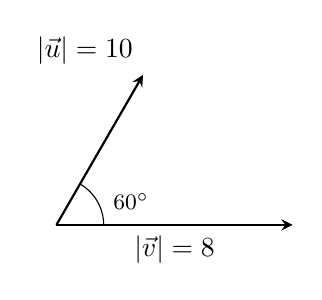
\begin{tikzpicture}[scale=1, >=stealth]
        \draw[->,thick] (0,0) -- (3,0) node[midway,below]{$|\vec{v}|=8$};
        \draw[->,thick] (0,0) -- ({2.2*cos(60)},{2.2*sin(60)}) node[above left]{$|\vec{u}|=10$};
        \draw (0.6,0) arc[start angle=0, end angle=60, radius=0.6];
        \node at (0.95,0.3) {\footnotesize $60^\circ$};
    \end{tikzpicture}
    \end{center}

    \item (Stewart \S12.4 \#15) Find $|\vec{u}\times\vec{v}|$ and determine whether $\vec{u}\times\vec{v}$ is directed into or out of the page.
    \begin{center}
    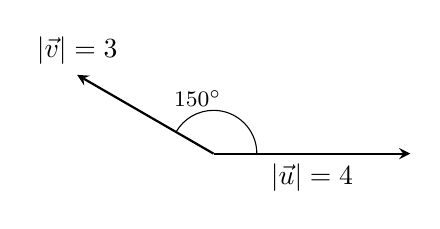
\begin{tikzpicture}[scale=1, >=stealth]
        \draw[->,thick] (0,0) -- (2.5,0) node[midway,below]{$|\vec{u}|=4$};
        \draw[->,thick] (0,0) -- ({2*cos(150)},{2*sin(150)}) node[above]{$|\vec{v}|=3$};
        \draw (0.55,0) arc[start angle=0, end angle=150, radius=0.55];
        \node at (-0.2,0.7) {\footnotesize $150^\circ$};
    \end{tikzpicture}
    \end{center}

    \item (Stewart \S12.4 \#16) The figure shows a vector $\vec{a}$ in the $xy$-plane and a vector $\vec{b}$ in the direction of $\khat$. Their lengths are $|\vec{a}|=3$ and $|\vec{b}|=2$.
    \begin{center}
    \begin{tikzpicture}[scale=1.0, >=stealth,
        x={(1cm,0cm)}, y={(-0.5cm,-0.4cm)}, z={(0cm,1cm)}]
        \draw[->] (0,0,0) -- (3.5,0,0) node[right]{$x$};
        \draw[->] (0,0,0) -- (0,3.5,0) node[below right]{$y$};
        \draw[->] (0,0,0) -- (0,0,3) node[above]{$z$};
        \draw[->,thick,blue] (0,0,0) -- (2.1,2.1,0) node[below]{$\vec{a}$};
        \draw[->,thick,red]  (0,0,0) -- (0,0,2) node[left]{$\vec{b}$};
    \end{tikzpicture}
    \end{center}
    (a) Find $|\vec{a}\times\vec{b}|$.\quad (b) Use the right-hand rule to decide whether each component of $\vec{a}\times\vec b$ is positive, negative, or zero.

    \item A torque wrench grips a bolt at the origin. The wrench is $30$ cm long, lies in the $xy$-plane, and points along $\langle 1,1,0\rangle/\sqrt{2}$. A downward force of magnitude $80$ N is applied at the far end.
    \begin{center}
    \begin{tikzpicture}[scale=1.0, >=stealth,
        x={(1cm,0cm)}, y={(-0.5cm,-0.4cm)}, z={(0cm,1cm)}]
        \draw[->] (0,0,0) -- (3.5,0,0) node[right]{$x$};
        \draw[->] (0,0,0) -- (0,3.5,0) node[below right]{$y$};
        \draw[->] (0,0,0) -- (0,0,2.5) node[above]{$z$};
        \draw[line width=2pt,gray] (0,0,0) -- (2.1,2.1,0);
        \fill (2.1,2.1,0) circle (2pt);
        \draw[->,thick,red] (2.1,2.1,0) -- (2.1,2.1,-1.8) node[right]{$\vec{F}$};
        \node[above left] at (1.1,1.1,0) {wrench};
    \end{tikzpicture}
    \end{center}
    Compute the torque vector $\vec\tau = \vec{r}\times\vec{F}$, its magnitude, and its direction.
    \item Compute $\langle 1,2,3\rangle\times\langle 4,5,6\rangle$ and verify it is orthogonal to both factors.
    \item Find the area of the triangle with vertices $(1,0,0)$, $(0,2,0)$, $(0,0,3)$.
    \item Find a unit vector orthogonal to both $\langle 1,1,0\rangle$ and $\langle 0,1,1\rangle$.
    \item Find the volume of the parallelepiped with edges $\langle 1,0,0\rangle$, $\langle 1,1,0\rangle$, $\langle 1,1,1\rangle$.
    \item Use the scalar triple product to decide whether $\langle 1,2,1\rangle$, $\langle 0,1,2\rangle$, and $\langle 2,3,0\rangle$ are coplanar.
\end{enumerate}

\subsection{Lines and Planes}

\subsubsection{Lines in Space}
\begin{enumerate}
    \item \dimtag{1D in 3D} (Stewart \S12.5 \#1) Determine whether each statement is true or false in $\mathbb{R}^3$.
    \begin{enumerate}
        \item Two lines parallel to a third line are parallel.
        \item Two lines perpendicular to a third line are parallel.
        \item Two planes parallel to a third plane are parallel.
        \item Two planes perpendicular to a third plane are parallel.
        \item Two lines parallel to a plane are parallel.
        \item Two lines perpendicular to a plane are parallel.
        \item Two planes parallel to a line are parallel.
        \item Two planes perpendicular to a line are parallel.
        \item Two planes either intersect or are parallel.
        \item Two lines either intersect or are parallel.
        \item A plane and a line either intersect or are parallel.
    \end{enumerate}
    \item (Stewart \S12.5 \#2) Find a vector equation and parametric equations for the line through $(4,2,-3)$ and parallel to $2\ihat - \jhat + 6\khat$.
    \item (Stewart \S12.5 \#4) Find a vector equation and parametric equations for the line through $(6,0,-2)$ and parallel to the line $x=4-3t,\ y=-1+4t,\ z=6+5t$.
    \item Find the parametric and symmetric equations of the line through $(2,1,0)$ that is perpindicular to both of $\langle 1,1,0 \rangle$ and $\langle 0,1,1 \rangle$.
    \item (Stewart \S12.5 \#10) Find parametric and symmetric equations for the line through $(2,1,0)$ and perpendicular to both $\ihat + \jhat$ and $\jhat + \khat$.
    \item The parametric equations $x = 3 + 2t$, $y = -1 - t$, $z = 4 + 3t$ describe a line. Write this line in vector form $\vec{r}(t) = \vec{r}_0 + t\vec{v}$, identifying the initial point $\vec{r}_0$ and direction vector $\vec{v}$.
    \item The symmetric equations of a line are given in the non-standard form $\dfrac{x-1}{2} = 3(y+2) = \dfrac{z}{-1}$. Identify a point on the line and a direction vector, then rewrite in standard symmetric form.
    \item (Stewart \S12.5 \#5) Find parametric and symmetric equations for the line through $(5,7,1)$ that is perpendicular to the plane $3x - 2y + 2z = 8$.
    \item Find the distance from the point $P(1, 0, -1)$ to the line given by the parametric equations $x = 2 + t, \ y = 1 - 2t, \ z = 3t$.
    \item Find parametric and symmetric equations of the line through $(2,1,0)$ and $(1,3,-2)$.
    \item Find parametric equations of the line through $(1,0,6)$ perpendicular to the plane $x+3y+z=5$.
    \item Decide whether the lines $\vec r_1=\langle 1+t,\,2t,\,3-t\rangle$ and $\vec r_2=\langle 2-s,\,3+s,\,1+2s\rangle$ are parallel, intersecting, or skew.
    \item Find the point where the line $x=1+t,\ y=2-t,\ z=3t$ meets the plane $x+y+z=6$.
\end{enumerate}

\subsubsection{Planes}
\begin{enumerate}
    \item \dimtag{2D in 3D} (Stewart \S12.5 \#24) Find an equation of the plane through $(-3,4,2)$ with normal vector $\langle 6,1,-1\rangle$.
    \item (Stewart \S12.5 \#26) Find an equation of the plane through the origin and perpendicular to the line $x = 1 - 8t,\ y = -1 - 7t,\ z = 4 + 2t$.
    \item Find an equation of the plane that passes through the points $P(1, 3, 2)$, $Q(3, -1, 6)$, and $R(5, 2, 0)$.
    \item (Stewart \S12.5 \#32) Find an equation of the plane through the origin and the points $(3,-2,1)$ and $(1,1,1)$.
    \item Find the equation of the plane through the origin that is parallel to the vectors $\vec{u} = \langle 1, -1, 2 \rangle$ and $\vec{v} = \langle 2, 1, -1 \rangle$.
    \item Find the distance from the point $Q(4, 1, -2)$ to the plane defined by the equation $2x - 3y + z = 10$.
    \item Find the point of intersection of the line $x=1+t,\ y=2-t,\ z=3t$ and the plane $2x+y-z=5$.
    \item (Stewart \S12.5 \#45) Find the point at which the line $x=2-2t,\ y=3t,\ z=1+t$ intersects the plane $x + 2y - z = 7$.
    \item Find the line of intersection of the planes $x + y + z = 1$ and $x + 2y + 2z = 1$.
    \item (Stewart \S12.5 \#12) Find parametric and symmetric equations for the line of intersection of the planes $x + 2y + 3z = 1$ and $x - y + z = 1$.
    \item (Stewart \S12.5 \#57) For the planes $x+y+z=1$ and $x+2y+2z=1$, do the following.
    \begin{enumerate}
        \item Find parametric equations for the line of intersection.
        \item Find the angle, in degrees rounded to one decimal place, between the planes.
    \end{enumerate}
    \item (Stewart \S12.5 \#44) Use intercepts to help sketch the plane $6x + 5y - 3z = 15$.
    \item The figure shows a plane $\Pi$ with normal $\vec{n}$ and a point $Q$ not on $\Pi$. Use the picture to derive the formula for the distance from $Q$ to $\Pi$ in terms of $\vec{n}$ and any point $P_0\in\Pi$.
    \begin{center}
    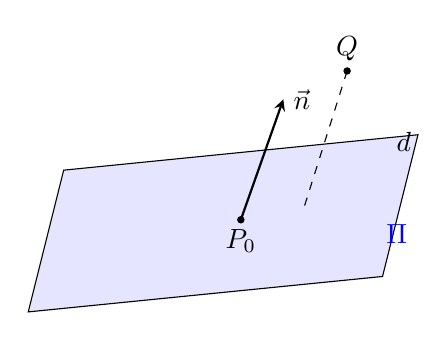
\begin{tikzpicture}[scale=0.9, >=stealth]
        \fill[blue!10] (-2,-1) -- (3,-0.5) -- (3.5,1.5) -- (-1.5,1) -- cycle;
        \draw (-2,-1) -- (3,-0.5) -- (3.5,1.5) -- (-1.5,1) -- cycle;
        \fill (1,0.3) circle (1.5pt) node[below]{$P_0$};
        \draw[->,thick] (1,0.3) -- (1.6,2) node[right]{$\vec{n}$};
        \fill (2.5,2.4) circle (1.5pt) node[above]{$Q$};
        \draw[dashed] (2.5,2.4) -- (1.9,0.5);
        \node at (3.3,1.4) {$d$};
        \node[blue] at (3.2,0.1) {$\Pi$};
    \end{tikzpicture}
    \end{center}
    \item Find an equation of the plane through $(1,2,3)$ with normal $\langle 2,-1,4\rangle$.
    \item Find an equation of the plane through $(1,0,0)$, $(0,2,0)$, and $(0,0,3)$.
    \item Find the angle between the planes $x+y+z=1$ and $x-2y+3z=1$.
    \item Find parametric equations for the line of intersection of $x+y+z=1$ and $x-y+2z=0$.
    \item Find the distance from $(1,1,1)$ to the plane $2x+2y+z=6$.
    \item Decide whether the planes $2x-3y+z=4$ and $-4x+6y-2z=1$ are parallel, and if so find the distance between them.
\end{enumerate}

\subsection{Quadric Surfaces (Graphing)}
\begin{enumerate}
    \item \dimtag{2D in 3D} Sketch the paraboloid surface $z = x^2 + y^2$. Sketch the curve formed by the intersection of this surface and the vertical plane $y=x$.
    \item Sketch the quadric surface defined by the equation $\frac{x^2}{4} + y^2 + \frac{z^2}{9} = 1$.
    \item Sketch the surface $x^2 + y^2 - z^2 = 1$. Identify and label the traces in the $xy$-plane and the $xz$-plane.
    \item For the quadric surface $\frac{x^2}{9} - \frac{y^2}{4} + \frac{z^2}{1} = 1$, do the following.
    \begin{enumerate}
        \item Find the traces in all three coordinate planes ($z=0$, $y=0$, $x=0$) and identify each as a conic section (ellipse, hyperbola, or parabola).
        \item Use the traces to identify and sketch the surface.
    \end{enumerate}
    \item For each surface below, find the traces parallel to each coordinate plane, identify the type of quadric, and sketch it.
    \begin{enumerate}
        \item $4x^2 + y^2 + z^2 = 16$
        \item $z = 4x^2 + y^2$
    \end{enumerate}
    \item Sketch the surface given by $z = y^2 - x^2$.
    \item Sketch the graph of the function $f(x,y) = \sqrt{1-x^2-y^2}$. Label at least 3 significant points.
    \item Sketch the surface $z = \sqrt{x^2 + y^2}$ and identify its intersection with the plane $z=2$.
    \item Identify and describe the traces of $\dfrac{x^2}{4}+\dfrac{y^2}{9}+z^2=1$.
    \item Name the surface $z=x^2+y^2$ and describe its horizontal and vertical traces.
    \item Name each surface: $z^2=x^2+y^2$, \ $x^2+y^2-z^2=1$, \ and $4x^2-y^2+2z^2=4$.
    \item Reduce $x^2+4y^2-z^2+2x=3$ by completing the square and name the quadric.
\end{enumerate}

\newpage
\center{\section{Exam 2 Material}}

\subsection{Space Curves and Vector Functions}

\subsubsection{Graphing and Parameterization}
\begin{enumerate}
    \item \dimtag{1D in 3D} (Stewart \S13.1 \#1) Find the domain of $\vec{r}(t) = \left\langle \ln(t+1),\ \dfrac{t}{\sqrt{9-t^2}},\ 2^t \right\rangle$.
    \item Let $\vec{r}(t) = \langle \ln(t-1),\ \arctan(t),\ \sqrt{4 - t^2} \rangle$.
    \begin{enumerate}
        \item Find the domain of $\vec{r}(t)$.
        \item Sketch the projection of the curve onto the $xy$-plane for $t$ in the domain.
        \item Indicate the direction of increasing $t$ with arrows on your sketch.
    \end{enumerate}
    \item (Stewart \S13.1 \#4) Evaluate
    \[ \lim_{t\to 1} \left\langle \frac{t^2-t}{t-1},\ \sqrt{t+8},\ \frac{\sin(\pi t)}{\ln t} \right\rangle. \]
    \item Sketch the directed curve $\vec{r}(t) = \langle 3\cos(t), 3\sin(t), 2 \rangle$ for $0 \leq t \leq 2\pi$. Indicate the direction of motion with an arrow.
    \item (Stewart \S13.1 \#8) Sketch the curve $\vec r(t) = \langle t^2 - 1, t\rangle$ and indicate with an arrow the direction in which $t$ increases.
    \item Sketch the curve $\vec{r}(t) = \langle t^2, t \rangle$ in 2D and describe its shape.
    \item (Stewart \S13.1 \#9) Sketch the curve $\vec r(t) = \langle 3\sin t,\ 2\cos t\rangle$ and indicate the direction in which $t$ increases.
    \item (Stewart \S13.1 \#10) Sketch the curve $\vec r(t) = e^t\,\ihat + e^{-t}\,\jhat$ for $t\in\mathbb{R}$.
    \item (Stewart \S13.1 \#11) Sketch the curve $\vec r(t) = \langle t,\ 2-t,\ 2t\rangle$.
    \item (Stewart \S13.1 \#12) Sketch $\vec r(t) = \langle \sin(\pi t),\ t,\ \cos(\pi t)\rangle$.
    \item (Stewart \S13.1 \#13) Sketch $\vec r(t) = \langle 3,\ t,\ 2 - t^2 \rangle$.
    \item Sketch the curve of intersection of the cylinder $x^2 + y^2 = 1$ and the plane $z = y + 1$. Provide a vector-valued function $\vec{r}(t)$ that represents this curve.
    \item Sketch the curve $\vec{r}(t) = \langle t\cos(t), t\sin(t), t \rangle$ for $t \geq 0$. Describe the surface upon which this curve lies.
    \item Graph the intersection of the sphere $x^2 + y^2 + z^2 = 4$ and the cylinder $(x-1)^2 + y^2 = 1$. Find a parameterization $\vec{r}(t)$ for this curve.
    \item Consider the vector function $\vec{r}(t) = \langle e^t \cos t,\ e^t \sin t \rangle$.
    \begin{enumerate}
        \item State the domain of $\vec{r}(t)$.
        \item Sketch the directed curve for $0 \leq t \leq 2\pi$, marking the points $\vec{r}(0)$, $\vec{r}(\pi/2)$, $\vec{r}(\pi)$. What happens to $|\vec{r}(t)|$ as $t$ increases?
    \end{enumerate}
    \item (Stewart \S13.1 \#25--29) For each set of parametric equations below, sketch the curve by hand and identify a simple surface (cone, cylinder, sphere, paraboloid, etc.) that contains it.
    \begin{enumerate}
        \item $x = t\cos t,\ y = t,\ z = t\sin t$,\ $t\geq 0$ \quad (\#25)
        \item $x = \cos t,\ y = \sin t,\ z = 1/(1+t^2)$ \quad (\#26)
        \item $x = t,\ y = 1/(1+t^2),\ z = t^2$ \quad (\#27)
        \item $x = \cos t,\ y = \sin t,\ z = \cos 2t$ \quad (\#28)
        \item $x = \cos 8t,\ y = \sin 8t,\ z = e^{0.8t},\ t\geq 0$ \quad (\#29)
    \end{enumerate}
    \item (Stewart \S13.1 \#39) At what points does the curve $\vec r(t) = t\,\ihat + (2t - t^2)\khat$ intersect the paraboloid $z = x^2 + y^2$?
    \item (Stewart \S13.1 \#58) Two particles travel along the curves
    \[ \vec r_1(t) = \langle t,\ t^2,\ t^3\rangle, \qquad \vec r_2(t) = \langle 1+2t,\ 1+6t,\ 1+14t\rangle. \]
    Do the particles collide? Do their paths intersect?

    \item The diagram below shows several level curves of an unknown function $f(x,y)$. Use it to estimate (i) the value of $f$ at $(1,1)$, (ii) the direction in which $f$ increases fastest from $(1,1)$, and (iii) whether $\partial f / \partial x$ at $(1,1)$ is positive, negative, or zero.
    \begin{center}
    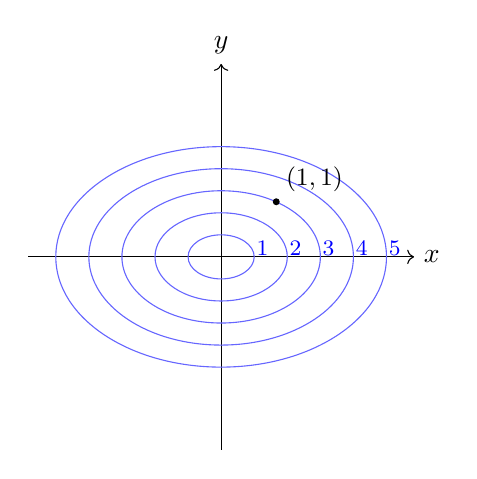
\begin{tikzpicture}[scale=0.7]
        \draw[->] (-3.5,0) -- (3.5,0) node[right]{$x$};
        \draw[->] (0,-3.5) -- (0,3.5) node[above]{$y$};
        \foreach \k in {1,2,3,4,5} {
            \draw[blue!60] (0,0) ellipse ({0.6*\k} and {0.4*\k});
            \node[blue,font=\footnotesize] at ({0.6*\k+0.15},0.15) {\k};
        }
        \fill (1,1) circle (1.8pt) node[above right]{\small $(1,1)$};
    \end{tikzpicture}
    \end{center}
    \item Find the domain of $\vec r(t)=\langle \ln t,\ \sqrt{4-t^2},\ 1/t\rangle$.
    \item Evaluate $\displaystyle\lim_{t\to 0}\Big\langle e^{2t},\ \tfrac{\sin t}{t},\ \cos t\Big\rangle$.
    \item Find a vector equation for the curve of intersection of the cylinder $x^2+y^2=4$ and the plane $z=x+1$.
    \item Name and sketch the curve $\vec r(t)=\langle \cos t,\ \sin t,\ t\rangle$.
\end{enumerate}

\subsubsection{Derivatives, Integrals, Velocity and Acceleration}
\begin{enumerate}
    \item \dimtag{1D in 3D} Given the position vector $\vec{r}(t) = \langle t^2, \sin(t), e^t \rangle$, find the velocity $\vec{v}(t)$ and acceleration $\vec{a}(t)$ at $t = 0$.
    \item (Stewart \S13.2 \#1) The figure shows a curve $C$ given by a vector function $\vec r(t)$, with the tip of $\vec r(4)$ at $P$, the tip of $\vec r(4.2)$ at $Q$, and the tip of $\vec r(4.5)$ at $R$.
    \begin{center}
    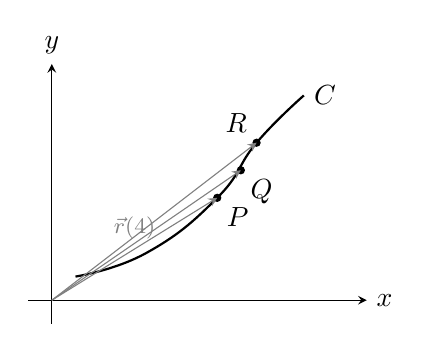
\begin{tikzpicture}[scale=1, >=stealth]
        \draw[->] (-0.3,0) -- (4,0) node[right]{$x$};
        \draw[->] (0,-0.3) -- (0,3) node[above]{$y$};
        \draw[thick] plot[smooth,tension=0.8] coordinates {(0.3,0.3) (1.2,0.6) (2.1,1.3) (2.6,2.0) (3.2,2.6)} node[right]{$C$};
        \fill (2.1,1.3) circle (1.5pt) node[below right]{$P$};
        \fill (2.4,1.65) circle (1.5pt) node[below right]{$Q$};
        \fill (2.6,2.0) circle (1.5pt) node[above left]{$R$};
        \draw[->,gray] (0,0) -- (2.1,1.3) node[midway,above]{\footnotesize $\vec r(4)$};
        \draw[->,gray] (0,0) -- (2.4,1.65);
        \draw[->,gray] (0,0) -- (2.6,2.0);
    \end{tikzpicture}
    \end{center}
    (a) Draw $\vec r(4.5)-\vec r(4)$ and $\vec r(4.2)-\vec r(4)$.\
    (b) Draw $\dfrac{\vec r(4.5)-\vec r(4)}{0.5}$ and $\dfrac{\vec r(4.2)-\vec r(4)}{0.2}$.\
    (c) Write expressions for $\vec r\,'(4)$ and the unit tangent $\vec T(4)$.\
    (d) Draw $\vec T(4)$.
    \item (Stewart \S13.2 \#3) For $\vec r(t) = \langle t - 2,\ t^2 + 1\rangle$ at $t = -1$, do three things. (a) Sketch the plane curve. (b) Find $\vec r\,'(t)$. (c) Sketch the position vector and tangent vector at the given $t$.
    \item (Stewart \S13.2 \#7) For $\vec r(t) = 4\sin t\,\ihat - 2\cos t\,\jhat$ at $t = 3\pi/4$, do three things. (a) Sketch the curve. (b) Find $\vec r\,'(t)$. (c) Sketch position and tangent.
    \item (Stewart \S13.2 \#39) Evaluate
    \[ \int_0^1 \left( \frac{1}{t+1}\,\ihat + \frac{1}{t^2+1}\,\jhat + \frac{t}{t^2+1}\,\khat \right) dt. \]
    \item (Stewart \S13.2 \#43) Find $\vec r(t)$ if $\vec r\,'(t) = 2t\,\ihat + 3t^2\,\jhat + \sqrt{t}\,\khat$ and $\vec r(1) = \ihat + \jhat$.
    \item Find the unit tangent vector $\vec{T}(t)$ and the unit normal vector $\vec{N}(t)$ for the helix $\vec{r}(t) = \langle \cos(t), \sin(t), t \rangle$.
    \item Find the tangential and normal components of acceleration ($a_T$ and $a_N$) for the curve $\vec{r}(t) = \langle t, t^2, 3t \rangle$.
    \item (Stewart \S13.4 \#3) Find the velocity, acceleration, and speed of a particle with position function $\vec r(t) = \langle -\tfrac12 t^2,\ t\rangle$ at $t = 2$. Sketch the path and draw the velocity and acceleration vectors at $t=2$.
    \item (Stewart \S13.4 \#10) Find the velocity, acceleration, and speed of a particle with position function $\vec r(t) = \langle 2\cos t,\ 3t,\ 2\sin t\rangle$.
    \item (Stewart \S13.4 \#16) Find the velocity and position vectors of a particle with $\vec a(t) = \sin t\,\ihat + 2\cos t\,\jhat + 6t\,\khat$, $\vec v(0) = -\khat$, $\vec r(0) = \jhat - 4\khat$.
    \item (Stewart \S13.4 \#35) A particle has position function $\vec r(t)$. If $\vec r\,'(t) = \vec c \times \vec r(t)$ where $\vec c$ is a constant vector, describe the path of the particle.
    \item (Stewart \S13.4 \#36) (a) If a particle moves along a straight line, what can you say about its acceleration vector? (b) If a particle moves with constant speed along a curve, what can you say about its acceleration vector?
    \item (Stewart \S13.4 \#37) Find the tangential and normal components of the acceleration vector for $\vec r(t) = (t^2+1)\,\ihat + t^3\,\jhat$, $t\geq 0$.
    \item If a particle moves with constant speed, prove that the velocity and acceleration vectors are always orthogonal.
    \item A particle moves such that its position vector $\vec{r}(t)$ always has a constant magnitude $R$. Show that the velocity vector $\vec{v}(t)$ is always perpendicular to $\vec{r}(t)$.
    \item A projectile is fired with an initial speed of 500 m/s at an angle of 30 degrees.  Find the range of the projectile.
     \item An electron moves through a magnetic field with a velocity vector at time $t$ in nanoseconds given by
    \[ \vec{v}(t) = \langle -\sin(t), \frac{1}{\sqrt{2}}\cos(t), \frac{1}{\sqrt{2}}\cos(t) \rangle \]
    At time $t=0$, the electron is located at the initial position $\vec{r}(0) = \langle 1, 0, 0 \rangle$.
    \begin{enumerate}
        \item Determine the position vector $\vec{r}(t)$ for all $t \geq 0$.
        \item Show that the electron is trapped on the surface of a sphere centered at the origin by finding the equation of that sphere.
    \end{enumerate}
    \item Find parametric equations of the tangent line to $\vec r(t)=\langle t,\ t^2,\ t^3\rangle$ at $t=1$.
    \item Evaluate $\displaystyle\int_0^1 \langle 2t,\ 3t^2,\ \sqrt{t}\rangle\,dt$.
    \item Find $\vec r(t)$ given $\vec r\,'(t)=\langle \sin t,\ -\cos t,\ 2t\rangle$ and $\vec r(0)=\langle 1,0,0\rangle$.
    \item Find the velocity, speed, and acceleration of $\vec r(t)=\langle t^2,\ e^{t},\ t\rangle$ at $t=0$.
    \item A projectile has acceleration $\langle 0,0,-g\rangle$, initial velocity $\langle v_0,0,0\rangle$, and starts at the origin. Find its position $\vec r(t)$.
\end{enumerate}

\subsubsection{Arc Length and Curvature}
\begin{enumerate}
    \item \dimtag{1D in 3D} (Stewart \S13.3 \#1) For $\vec r(t) = \langle 3-t,\ 2t,\ 4t+1\rangle$, $1\leq t \leq 3$, do two things. (a) Use the arc length integral to compute the length of the segment. (b) Compute the length using the distance formula and compare.
    \item (Stewart \S13.3 \#3) Find the length of $\vec r(t) = \langle t,\ 3\cos t,\ 3\sin t\rangle$ for $-5 \leq t \leq 5$.
    \item Find the length of the arc of the circular helix $\vec{r}(t) = \langle \cos(t), \sin(t), t \rangle$ from $t=0$ to $t=2\pi$.
    \item (Stewart \S13.3 \#20) For $\vec r(t) = \langle 5\sin t,\ t,\ 5\cos t\rangle$, do two things. (a) Find the unit tangent vector $\vec T(t)$ and unit normal $\vec N(t)$. (b) Find the curvature.
    \item (Stewart \S13.3 \#21) For $\vec r(t) = \langle t,\ t^2,\ 4\rangle$, find $\vec T(t)$, $\vec N(t)$, and $\kappa(t)$.
    \item Calculate the curvature $\kappa(t)$ for the space curve $\vec{r}(t) = \langle t, t^2, \frac{2}{3}t^3 \rangle$ using the formula $\kappa = \frac{|\vec{r}' \times \vec{r}''|}{|\vec{r}'|^3}$.
    \item Find the point on the curve $y = e^x$ where the curvature is maximized.
    \item Find the curvature of the parabola $y = x^2$ at the origin.
    \item Consider the ellipse $\frac{x^2}{4} + y^2 = 1$.
    \begin{enumerate}
        \item Compute the curvature $\kappa$ at the points $(2, 0)$ and $(0, 1)$.
        \item For each point, find the radius of curvature $\rho = 1/\kappa$ and the center of the osculating circle. (The center lies at distance $\rho$ from the point in the direction of $\vec{N}$.)
        \item Sketch the ellipse and both osculating circles. At which point is the ellipse curving more sharply?
    \end{enumerate}
    \item Find the curvature of $\vec{r}(t) = \langle 2\cos t, 3\sin t, 0 \rangle$ at $t = 0$ and $t = \pi/2$. Sketch the curve and draw the osculating circles at these two points.
    \item Find the length of $\vec r(t)=\langle 2t,\ t^2,\ \tfrac13 t^3\rangle$ for $0\le t\le 1$.
    \item Find the curvature of $y=x^2$ at the origin and at $(1,1)$.
    \item Find the unit tangent $\vec T$ and unit normal $\vec N$ for $\vec r(t)=\langle \cos t,\ \sin t\rangle$.
    \item Find the radius of the osculating circle of $y=\ln x$ at $(1,0)$.
\end{enumerate}

\subsection{Functions of Multiple Variables}

\subsubsection{Domains and Level Sets}
\begin{enumerate}
    \item \dimtag{2D in 3D} Sketch the level curves of $f(x,y) = x^2 + 4y^2$ for the values $k=1, k=4, k=9$.
    \item Sketch the domain of the function $f(x,y) = \ln(y - x^2)$.
    \item Describe the level surfaces of $f(x,y,z) = x^2 - y^2 - z^2$ for $k > 0$, $k = 0$, and $k < 0$.
    \item Sketch the level curves for $f(x,y) = \frac{x}{x^2 + y^2}$. Show that these curves are all circles.
    \item Sketch three level surfaces of the function $f(x,y,z) = x^2 + y^2 + z^2$.
    \item (Stewart \S14.1 \#36) Two contour maps below are shown. One belongs to a function whose graph is a cone, the other to a function whose graph is a paraboloid. Decide which is which and justify your answer.
    \begin{center}
    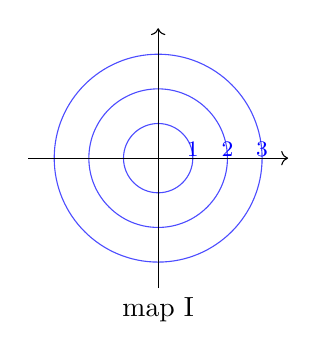
\begin{tikzpicture}[scale=0.55]
        \foreach \r in {0.8,1.6,2.4} \draw[blue!70] (0,0) circle (\r);
        \foreach \r/\lbl in {0.8/1, 1.6/2, 2.4/3}
            \node[blue,font=\footnotesize] at (\r,0.2) {\lbl};
        \draw[->] (-3,0)--(3,0); \draw[->] (0,-3)--(0,3);
        \node at (0,-3.5) {map I};
    \end{tikzpicture}\hspace{1.5cm}%
    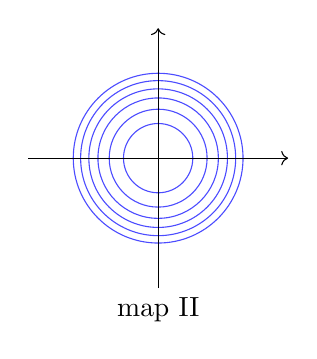
\begin{tikzpicture}[scale=0.55]
        \foreach \r/\lbl in {0.8/1, 1.13/2, 1.39/3, 1.6/4, 1.79/5, 1.96/6}
            \draw[blue!70] (0,0) circle (\r);
        \draw[->] (-3,0)--(3,0); \draw[->] (0,-3)--(0,3);
        \node at (0,-3.5) {map II};
    \end{tikzpicture}
    \end{center}
    (Level sets in map I are evenly spaced. In map II they bunch up as the radius grows.)
    \item (Stewart \S14.1 \#37, adapted) The topographic map below shows a feature called ``Lonesome Mountain.'' Consider the marked points $A$ (on the western flank, where contours are closely spaced) and $B$ (between two rings on the eastern ridge). Describe in words the shape of the terrain near each.
    \begin{center}
    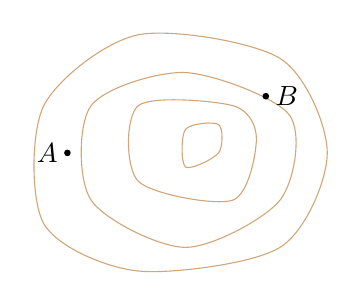
\begin{tikzpicture}[scale=0.6]
        \draw[brown!70] plot[smooth cycle] coordinates {(-3,-1.5) (-1,-2.5) (2,-2) (3,0) (2,2) (-1,2.5) (-3,1)};
        \draw[brown!70] plot[smooth cycle] coordinates {(-2,-1) (0,-2) (2,-1) (2.2,0.8) (0,1.7) (-2,1)};
        \draw[brown!70] plot[smooth cycle] coordinates {(-1,-0.6) (1,-1) (1.5,0.3) (1,1) (-1,1)};
        \draw[brown!70] plot[smooth cycle] coordinates {(0,-0.3) (0.7,0) (0.7,0.6) (0,0.5)};
        \fill (-2.5,0) circle (2pt) node[left]{$A$};
        \fill (1.7,1.2) circle (2pt) node[right]{$B$};
    \end{tikzpicture}
    \end{center}
    \item Find and sketch the domain of $f(x,y)=\sqrt{9-x^2-y^2}$ and of $g(x,y)=\ln(x-y)$.
    \item Sketch several level curves of $f(x,y)=y-x^2$ and of $g(x,y)=x^2-y^2$.
    \item Describe the level surfaces of $f(x,y,z)=x^2+y^2+z^2$.
\end{enumerate}

\subsubsection{Limits and Continuity}
\begin{enumerate}
    \item \dimtag{2D} Evaluate the limit, or show it does not exist, for $\displaystyle \lim_{(x,y) \to (0,0)} \frac{x^2 - y^2}{x^2 + y^2}$.
    \item Use polar coordinates to evaluate $\displaystyle \lim_{(x,y) \to (0,0)} \frac{x^3 + y^3}{x^2 + y^2}$.
    \item Show that $\displaystyle \lim_{(x,y) \to (0,0)} \frac{x y^3}{x^2 + y^6}$ does not exist, even though the limit is $0$ along every straight line through the origin.
    \item Determine the set of points at which $f(x,y) = \frac{1}{1 - x^2 - y^2}$ is continuous.
    \item Show that the limit $\displaystyle \lim_{(x,y) \to (0,0)} \frac{5y^4 \cos^2 x}{x^4 + y^4}$ does not exist.
    \item (Stewart \S14.2 \#49) Let
    \[ f(x,y) = \begin{cases} \dfrac{x^2 y^3}{2x^2 + y^2} & (x,y)\neq (0,0)\\ 1 & (x,y) = (0,0)\end{cases}. \]
    Is $f$ continuous at the origin? Justify carefully.
    \item Show that $\displaystyle\lim_{(x,y)\to(0,0)}\frac{x^2-y^2}{x^2+y^2}$ does not exist.
    \item Show that $\displaystyle\lim_{(x,y)\to(0,0)}\frac{xy^2}{x^2+y^4}$ does not exist by comparing the paths $x=0$ and $x=y^2$.
    \item Evaluate $\displaystyle\lim_{(x,y)\to(0,0)}\frac{x^2 y}{x^2+y^2}$ or show it fails to exist.
    \item Where is $f(x,y)=\dfrac{x+y}{x-y}$ continuous?
\end{enumerate}

\subsubsection{Basic Partial Derivatives Practice}
\begin{enumerate}
    \item \dimtag{1D in 3D} Find $f_x$ and $f_y$ for $f(x, y) = x^4 y^2 - 10x^2 y + 7y - 3$.
    \item Find $f_x$ and $f_y$ for $f(x, y) = \sin(x^2 y + y^3)$.
    \item Find $f_x$ and $f_y$ for $f(x, y) = e^{xy} \ln(x^2 + 1)$.
    \item Find $f_x$ and $f_y$ for $f(x, y) = \frac{x+y}{x-y}$.
    \item Find $f_x$ and $f_y$ for $f(x, y) = \arctan(y/x)$.
    \item For $f(x, y) = e^{x} \sin(y)$, verify that $f_{xy} = f_{yx}$.
    \item (Stewart \S14.3 \#13) Find the first partial derivatives of $z = \ln(x + t^2)$ (treating $x$ and $t$ as the two independant variables).
    \item (Stewart \S14.3 \#14) Find the first partial derivatives of $w = u/v^2$.
    \item (Stewart \S14.3 \#16) Find the first partials of $g(x,y) = (x + xy^2)^3$.
    \item (Stewart \S14.3 \#19) Find the first partials of $f(x,y) = \dfrac{ax+by}{cx+dy}$.
    \item (Stewart \S14.3 \#26) Find the first partials of $F(\alpha,\beta) = \displaystyle\int_\alpha^\beta \sqrt{t^3 + 1}\, dt$.
    \item (Stewart \S14.3 \#37) For $R(s,t) = t\,e^{s/t}$, find $R_t(0,1)$.
    \item (Stewart \S14.3 \#46) Find $\partial z/\partial x$ and $\partial z/\partial y$ for each of the following.
    \begin{enumerate}
        \item $z = f(x)\,g(y)$
        \item $z = f(x+y)$
        \item $z = f(xy)$
        \item $z = f(x/y)$
    \end{enumerate}
    \item (Stewart \S14.3 \#4--5) The figure shows the graph of a function $f(x,y)$. The surface near the point $(\pm 1, 2)$ slopes down as $x$ increases (steeply on the left, gently on the right) and slopes slightly down as $y$ increases.
    \begin{center}
    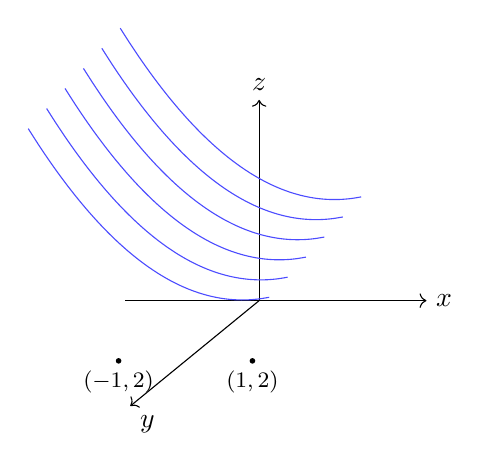
\begin{tikzpicture}[scale=0.85, x={(1cm,0cm)}, y={(-0.55cm,-0.45cm)}, z={(0cm,1cm)}]
        \draw[->] (-2,0,0)--(2.5,0,0) node[right]{$x$};
        \draw[->] (0,0,0)--(0,3.5,0) node[below right]{$y$};
        \draw[->] (0,0,0)--(0,0,3) node[above]{$z$};
        \foreach \yv in {0.5,1,1.5,2,2.5,3}{
            \draw[blue!70] plot[smooth,samples=25,domain=-1.8:1.8]
                (\x, \yv, {2.3 - 0.7*\x - 0.15*\yv + 0.25*\x*\x});
        }
        \fill (1,2,0) circle (1.2pt) node[below]{\footnotesize $(1,2)$};
        \fill (-1,2,0) circle (1.2pt) node[below]{\footnotesize $(-1,2)$};
    \end{tikzpicture}
    \end{center}
    Determine the sign of each. (a) $f_x(1,2)$, (b) $f_y(1,2)$, (c) $f_x(-1,2)$, (d) $f_y(-1,2)$.
    \item (Stewart \S14.3 \#6) A contour map of a function $f$ is shown below.
    \begin{center}
    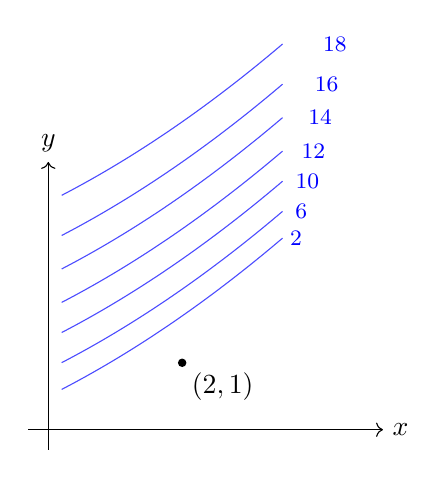
\begin{tikzpicture}[scale=0.85]
        \draw[->] (-0.3,0) -- (5,0) node[right]{$x$};
        \draw[->] (0,-0.3) -- (0,4) node[above]{$y$};
        \foreach \k/\sh in {2/0, 6/0.4, 10/0.85, 12/1.3, 14/1.8, 16/2.3, 18/2.9}{
            \draw[blue!70] plot[smooth,samples=40,domain=0.2:3.5]
                (\x, {0.5 + 0.5*\x + \sh + 0.05*\x*\x});
            \node[blue,font=\footnotesize] at (3.7+0.2*\sh, {0.5 + 0.5*3.5 + \sh + 0.05*3.5*3.5}) {\k};
        }
        \fill (2,1) circle (1.8pt) node[below right]{$(2,1)$};
    \end{tikzpicture}
    \end{center}
    Use the contour map to estimate $f_x(2,1)$ and $f_y(2,1)$.
    \item Let $V(r, h) = rh\cos(\frac{\pi}{2}e^{rh})$, where $r$ and $h$ are functions of time $t$ given by
    \[ r(t) = \cos^2(t), \quad h(t) = \sin(3t) \]
    Find $\frac{dV}{dt} |_{t=\pi}$.   
    \vspace{2mm} Consider the curve $\vec{p}(t) = ( \ r(t), \  h(t), \ V(r(t),h(t)) \ )$ along the graph of $V$. What does $\frac{dV}{dt} |_{t = \pi}$ represent in terms of $\vec{p}(t)$?
    \item Find $f_x$ and $f_y$ for $f(x,y)=x^3 y-2xy^2+y$.
    \item Find $f_x$ and $f_y$ for $f(x,y)=\ln(x^2+y^2)$ and for $g(x,y)=\dfrac{x}{x+y}$.
    \item Verify Clairaut's theorem $f_{xy}=f_{yx}$ for $f=x^3 y^2-2xy^4$.
    \item Find all second partial derivatives of $f(x,y)=x e^{y}+y e^{x}$.
    \item For $f(x,y,z)=xyz+x^2 z$, find $f_x$, $f_y$, and $f_z$.
\end{enumerate}

\subsubsection{Implicit Differentiation}
\begin{enumerate}
    \item \dimtag{2D in 3D} Find $\frac{\partial z}{\partial x}$ and $\frac{\partial z}{\partial y}$ for $x^2 + y^2 + z^2 = 3xyz$.
    \item Find $\frac{\partial z}{\partial x}$ and $\frac{\partial z}{\partial y}$ for $x e^y + y z + z e^x = 0$.
    \item Find $\frac{\partial z}{\partial x}$ and $\frac{\partial z}{\partial y}$ for $\sin(x+y) + \sin(y+z) + \sin(x+z) = 0$.
    \item Find $\partial z/\partial x$ and $\partial z/\partial y$ if $x^2+y^2+z^2=3xyz$.
    \item Find $\partial z/\partial x$ if $e^{z}=xyz$.
    \item Find $dy/dx$ for $x^2+xy+y^2=3$ using the ratio of partials of $F$.
\end{enumerate}

\subsubsection{Chain Rule Practice}
\begin{enumerate}
    \item \dimtag{1D in 3D} (Stewart \S14.5 \#3) Use the chain rule to find $dz/dt$, where $z = xy^3 - x^2 y$, $x = t^2 + 1$, $y = t^2 - 1$.
    \item (Stewart \S14.5 \#5) Find $dz/dt$ for $z = \sin x \cos y$, $x = \sqrt{t}$, $y = 1/t$.
    \item (Stewart \S14.5 \#6) Find $dw/dt$ for $w = \sqrt{1+xy}$, $x = \tan t$, $y = \arctan t$.
    \item (Stewart \S14.5 \#11) Find $\partial z/\partial s$ and $\partial z/\partial t$ for $z = (x-y)^5$, $x = s^2 t$, $y = st^2$.
    \item (Stewart \S14.5 \#13) Find $\partial z/\partial s$ and $\partial z/\partial t$ for $z = \ln(3x+2y)$, $x = s\sin t$, $y = t\cos s$.
    \item (Stewart \S14.5 \#15) Find $\partial z/\partial s$ and $\partial z/\partial t$ for $z = (\sin\theta)/r$, $r=st$, $\theta = s^2 + t^2$.
    \item (Stewart \S14.5 \#20) Suppose $f$ is a differentiable function of $x$ and $y$, and $g(r,s) = f(2r - s,\ s^2 - 4r)$. Using the table $f(1,2)=6,\ f_x(1,2)=2,\ f_y(1,2)=5$, calculate $g_r(1,2)$ and $g_s(1,2)$.
    \item (Stewart \S14.5 \#22) Use a tree diagram to write out the Chain Rule for the case $w = f(x,y,z)$, where $x = x(u,v),\ y = y(u,v),\ z = z(u,v)$.
    \item Given $w = f(x, y)$, where $x = s+t$ and $y = s-t$, show that $\frac{\partial w}{\partial s} + \frac{\partial w}{\partial t} = 2\frac{\partial f}{\partial x}$.
    \item Let $z = e^{xy} \cos(x+y)$, where $x = st$ and $y = s/t$. Find $\frac{\partial z}{\partial s}$.
    \item If $u = f(x-at) + g(x+at)$, show that $u$ satisfies the wave equation $\frac{\partial^2 u}{\partial t^2} = a^2 \frac{\partial^2 u}{\partial x^2}$.
    \item Let $z = x^2 y$, where $x = r\cos\theta$ and $y = r\sin\theta$. Find $\frac{\partial z}{\partial \theta}$ using the chain rule.
    \item If $z=x^2 y$, $x=t^2$, $y=t^3$, find $dz/dt$ two ways and compare.
    \item If $w=x^2+y^2+z^2$ with $x=\cos t$, $y=\sin t$, $z=t$, find $dw/dt$.
    \item If $z=e^{x}\sin y$ with $x=st$ and $y=s^2 t$, find $\partial z/\partial s$ and $\partial z/\partial t$.
    \item The radius of a cone grows at $2$ cm/s and its height shrinks at $3$ cm/s. Find the rate of change of the volume when $r=10$ and $h=20$.
\end{enumerate}

\subsubsection{Tangent Planes and Linearization}
\begin{enumerate}
    \item \dimtag{2D in 3D} Find an equation of the tangent plane to the surface $x^2 + 2y^2 + 3z^2 = 21$ at the point $(2, 2, 1)$.
    \item (Stewart \S14.4 \#2) Find an equation of the tangent plane to the surface $z = y^2 \sin x$ at the point $(\pi/2, -2, 4)$.
    \item (Stewart \S14.4 \#4) Find the tangent plane to $z = (x+2)^2 - 2(y-1)^2 - 5$ at $(2, 3, 3)$.
    \item (Stewart \S14.4 \#6) Find the tangent plane to $z = y^2 e^x$ at $(0, 3, 9)$.
    \item Find the linear approximation of $f(x,y) = \sqrt{20 - x^2 - 7y^2}$ at $(2, 1)$ and use it to estimate $f(1.95, 1.08)$.
    \item (Stewart \S14.4 \#15) Explain why $f(x,y) = x^3 y^2$ is differentiable at $(-2,1)$ and find the linearization $L(x,y)$ at that point.
    \item (Stewart \S14.4 \#18) Explain why $f(x,y) = \sqrt{xy}$ is differentiable at $(1,4)$, and find its linearization there.
    \item (Stewart \S14.4 \#22) Explain why $f(x,y) = y + \sin(x/y)$ is differentiable at $(0,3)$, and find its linearization there.
    \item Sketch the traces $z=f(x, y_0)$ and $z=f(x_0, y)$ and explain how they determine the tangent plane.
    \item Find the tangent plane to $z=x^2+y^2$ at $(1,1,2)$.
    \item Find the tangent plane to $z=\ln(2x+y)$ at $(-1,3,0)$.
    \item Find the linearization of $f(x,y)=\sqrt{x^2+y^2}$ at $(3,4)$ and use it to estimate $\sqrt{(3.02)^2+(3.9)^2}$.
    \item Find $dz$ for $z=x^2 y^3$ and use it to estimate the change as $(x,y)$ moves from $(1,2)$ to $(1.05,1.98)$.
\end{enumerate}

\subsubsection{Directional Derivatives and Gradients}
\begin{enumerate}
    \item \dimtag{2D in 3D} Find the directional derivative of $f(x,y) = x^2 y^3$ at $P(1, 2)$ in the direction of $\vec{v} = \ihat + \jhat$.
    \item (Stewart \S14.6 \#7) Find the directional derivative of $f(x,y) = \arctan(xy)$ at $(2,-3)$ in the direction indicated by the angle $\theta = 3\pi/4$.
    \item (Stewart \S14.6 \#9) For $f(x,y) = x/y$ at $P(2,1)$ with unit direction $\vec u = \tfrac{3}{5}\ihat + \tfrac{4}{5}\jhat$, do three things.
    (a) Find $\nabla f$. (b) Evaluate $\nabla f$ at $P$. (c) Find the rate of change of $f$ at $P$ in the direction $\vec u$.
    \item (Stewart \S14.6 \#10) Same parts (a)(b)(c) for $f(x,y) = x^2 \ln y$ at $P(3,1)$ with $\vec u = -\tfrac{5}{13}\ihat + \tfrac{12}{13}\jhat$.
    \item (Stewart \S14.6 \#14) Find the directional derivative of $f(x,y) = x/(x^2+y^2)$ at $(1,2)$ in the direction $\vec v = \langle 3,5\rangle$.
    \item (Stewart \S14.6 \#22) Find the directional derivative of $f(x,y) = x/y^2$ at $P(3,-1)$ in the direction of $Q(-2,11)$.
    \item Find the maximum rate of change of $f(x,y,z) = x + y/z$ at the point $(1, 1, 1)$ and the direction in which it occurs.
    \item (Stewart \S14.6 \#26) The contour map of a function $f$ is shown below. At each of the points $P,Q,R$, draw an arrow indicating the direction of the gradient vector.
    \begin{center}
    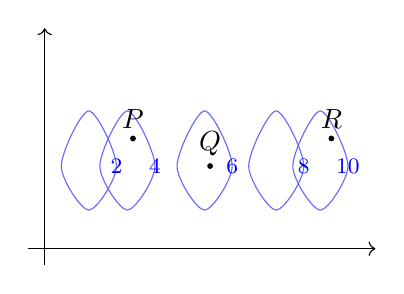
\begin{tikzpicture}[scale=0.7]
        \draw[->] (-0.3,0)--(6,0); \draw[->] (0,-0.3)--(0,4);
        \foreach \v/\h in {10/5.5, 8/4.7, 6/3.4, 4/2, 2/1.3}{
            \draw[blue!60] plot[smooth cycle] coordinates {(\h,1.5) (\h-0.5,2.5) (\h-1,1.5) (\h-0.5,0.7)};
            \node[blue,font=\footnotesize] at (\h,1.5) {\v};
        }
        \fill (1.6,2) circle (1.5pt) node[above]{$P$};
        \fill (3,1.5) circle (1.5pt) node[above]{$Q$};
        \fill (5.2,2) circle (1.5pt) node[above]{$R$};
    \end{tikzpicture}
    \end{center}
    \item (Stewart \S14.6 \#27) Find the maximum rate of change of $f(x,y) = 5xy^2$ at $(3,-2)$ and the direction in which it occurs.
    \item (Stewart \S14.6 \#33b) Use the fact that $f$ decreases most rapidly in the direction $-\nabla f$ to find the direction in which $f(x,y) = x^4 y - x^2 y^3$ decreases fastest at $(2,-3)$. What is the rate of decrease?
    \item (Stewart \S14.6 \#38) The temperature at a point $(x,y,z)$ is given by $T(x,y,z) = 200\,e^{-x^2 - 3y^2 - 9z^2}$.
    (a) Rate of change of $T$ at $P(2,-1,2)$ in the direction toward $(3,-3,3)$.
    (b) In which direction does $T$ increase fastest at $P$?
    (c) What is the maximum rate of increase at $P$?
    \item Show that the gradient vector $\nabla f(x_0, y_0, z_0)$ is always perpendicular to the level surface $f(x,y,z) = k$ at the point $(x_0, y_0, z_0)$.
    \item Find all points $(x,y)$ where the directional derivative of $f(x,y) = x^2 + y^2$ in the direction $\vec{u} = \langle 1/\sqrt{2}, 1/\sqrt{2} \rangle$ is zero.
    \item Sketch the level curves of $f(x,y) = x^2 + y^2$. At the point $(1,1)$, draw the gradient vector $\nabla f$.
    \item A solid object has a temperature distribution given by $F(x, y, z) = x^2 + 2y^2 + 3z^2$ (in degrees Celsius).
    \begin{enumerate}
        \item Show that the point $P(1, 2, 1)$ lies on the isothermal (constant temperature) surface $F(x, y, z) = 12$.
        \item Find the gradient vector $\nabla F$ at the point $P$.
        \item Find the equation of the tangent plane to this isothermal surface at point $P$.
        \item Heat flows in the direction of the greatest temperature change. At point $P$, for what unit vector $\hat{u}$ is the magnitude of the directional derivative $|D_{\hat{u}} F|$ the largest?
    \end{enumerate}
    \item Find $\nabla f$ for $f(x,y)=x^2 y-y^3$ and the directional derivative at $(2,1)$ in the direction of $\langle 3,4\rangle$.
    \item Find the maximum rate of change of $f(x,y)=\sin(xy)$ at $(1,0)$ and the direction in which it occurs.
    \item At $(1,2)$, in what direction does $f(x,y)=x^2+y^2$ decrease fastest, and in what directions is its rate of change zero?
    \item Find the tangent plane and the normal line to the level surface $x^2+2y^2+3z^2=6$ at $(1,1,1)$.
\end{enumerate}

\subsubsection{Maxima and Minima}
\begin{enumerate}
    \item \dimtag{2D in 3D} Find and classify the critical points of $f(x, y) = x^4 + y^4 - 4xy + 1$.
    \item (Stewart \S14.7 \#3) The level curves of $f(x,y) = 4 + x^3 + y^3 - 3xy$ are shown below, each contour labeled with its $f$-value. Predict the location of the critical points and whether each is a saddle, local max, or local min. Then use the Second Derivatives Test to confirm.
    \begin{center}
    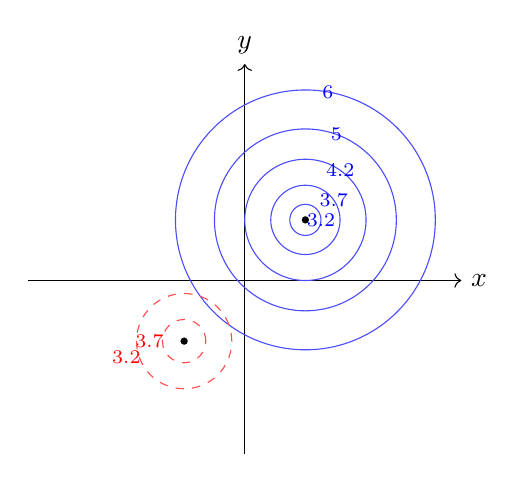
\begin{tikzpicture}[scale=1.1]
        \draw[->] (-2.5,0)--(2.5,0) node[right]{$x$};
        \draw[->] (0,-2)--(0,2.5) node[above]{$y$};
        \foreach \k/\r/\ang in {3.2/0.18/0, 3.7/0.4/35, 4.2/0.7/55, 5/1.05/70, 6/1.5/80}{
            \draw[blue!70] (0.7,0.7) circle (\r);
            \node[blue,font=\scriptsize] at ({0.7 + \r*cos(\ang)},{0.7 + \r*sin(\ang)}) {\k};
        }
        \foreach \k/\r/\ang in {3.7/0.25/180, 3.2/0.55/200}{
            \draw[red!70,dashed] (-0.7,-0.7) circle (\r);
            \node[red,font=\scriptsize] at ({-0.7 + \r*cos(\ang) - 0.15},{-0.7 + \r*sin(\ang)}) {\k};
        }
        \fill (0.7,0.7) circle (1.2pt);
        \fill (-0.7,-0.7) circle (1.2pt);
    \end{tikzpicture}
    \end{center}
    \item Find the absolute maximum and minimum of $f(x,y)=xy$ on the disk $x^2 + y^2 \le 1$.
    \item Find the shortest distance from the origin to the plane $x + 2y + 3z = 12$ using the Second Derivative Test.
     \item For $f(x,y) = x^2 + y^2 - 2x$, use the second derivative test to classify the critical points, then find the absolute maximum and absolute minimum values on the closed disk $x^2 + y^2 \leq 4$.
    \item Sketch a saddle point surface. Explain how the determinant of the Hessian $D < 0$ captures this behavior.
    \item Find 3 positive numbers whose sum is $100$ and whose product is a maximum.
    \item Find and classify the critical points of $f(x,y)=x^2+y^2-4x-6y+13$.
    \item \dimtag{1D in 2D} Classify the critical points of $g(x)=x^3-3x$ with the second derivative test, then do the same for $f(x,y)=x^3-3x+y^2$ and explain how the added $y^2$ turns the maximum into a saddle.
    \item Find and classify the critical points of $f(x,y)=x^4+y^4-4xy+1$.
    \item Find three positive numbers whose sum is $12$ and whose product is as large as possible.
    \item Find the point on the plane $x+2y+2z=6$ closest to the origin by minimizing the squared distance.
\end{enumerate}


\newpage
\center{\section{Exam 3 Material}}

\subsection{Multiple Integrals}

\subsubsection{The Dome as a Volume (running example)}
\begin{enumerate}
    \item \dimtag{1D} The companion curve is $y = 1 - x^2$ on $[-1,1]$, the dome's vertical slice through the $x$-axis. Sketch it and find the area under it, $\int_{-1}^{1}(1-x^2)\,dx$.
    \item \dimtag{2D in 3D} Sketch the dome over the unit disk and its shadow $x^2+y^2\le 1$. Set up the volume $\iint_D (1-x^2-y^2)\,dA$ with the inner strip in $y$. Read the limits off the shadow, but do not evaluate yet.
    \item \dimtag{2D in 3D} The same volume in polar is $\displaystyle\int_0^{2\pi}\!\int_0^1 (1-r^2)\,r\,dr\,d\theta$. Evaluate it, and say in one line why the extra $r$ appears and why polar is the honest coordinate for a disk.
    \item \dimtag{2D} Reverse the order of your rectangular integral from problem 2 and confirm the shadow is described the other way. Which order would you rather carry out, and why?
    \item \dimtag{3D} Sweep the solid vertically. Write the volume as $\iiint_E dV$ with $0\le z\le 1-x^2-y^2$ over the disk shadow, then redo it in cylindrical as $\displaystyle\int_0^{2\pi}\!\int_0^1\!\int_0^{1-r^2} r\,dz\,dr\,d\theta$. Check it matches problem 3.
    \item \dimtag{3D} Give the solid density $\delta = 1$. By symmetry $\bar x = \bar y = 0$. Find $\bar z = \frac{1}{V}\iiint_E z\,dV$ in cylindrical and mark the balance height on your sketch.
    \item \dimtag{3D} Cap the same disk with the hemisphere $z = \sqrt{1-x^2-y^2}$ instead of the dome. Set up its volume in spherical, $\displaystyle\int_0^{2\pi}\!\int_0^{\pi/2}\!\int_0^1 \rho^2\sin\phi\,d\rho\,d\phi\,d\theta$, and sketch the spherical wedge whose three edges give $\rho^2\sin\phi$. Compare the two solids over the shared shadow.
\end{enumerate}

\subsubsection{Double Integrals (Rectangular and General Regions)}
\begin{enumerate}
    \item \dimtag{2D} (Stewart \S15.1 \#2a) For $R = [0,4]\times[-1,2]$ and the integral $\iint_R (1 - xy^2)\,dA$, use a Riemann sum with $m=2$, $n=3$, sampling at the \emph{lower right} corner of each subrectangle.
    \item (Stewart \S15.1 \#4b) Use the Midpoint Rule with $m=n=2$ to estimate the volume under $z = 1 + x^2 + 3y$ above $R=[1,2]\times[0,3]$.
    \item (Stewart \S15.1 \#9) Evaluate $\iint_R \sqrt{2}\,dA$ where $R = \{(x,y) : 2\leq x\leq 6,\ -1\leq y \leq 5\}$ by first identifying it as the volume of a solid.
    \item (Stewart \S15.1 \#10) Evaluate $\iint_R (2x+1)\,dA$ where $R=\{(x,y): 0\leq x \leq 2,\ 0\leq y\leq 4\}$ by identifying it as a volume.
    \item (Stewart \S15.1 \#14) For $f(x,y) = y\sqrt{x+2}$, find $\int_0^2 f(x,y)\, dx$ and $\int_0^3 f(x,y)\,dy$.
    \item (Stewart \S15.1 \#7) A contour map of a function $f$ on the square $R=[0,4]\times[0,4]$ is shown below, each blue curve labeled with the corresponding value of $f$. Use the Midpoint Rule with $m=n=2$ to estimate $\iint_R f\,dA$, and estimate the average value of $f$.
    \begin{center}
    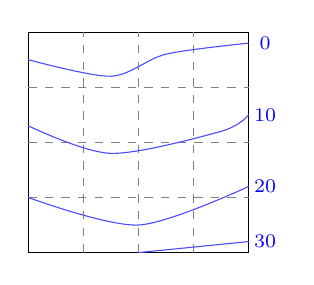
\begin{tikzpicture}[scale=0.7]
        \draw (0,0) rectangle (4,4);
        \foreach \x in {1,2,3} \draw[dashed,gray] (\x,0)--(\x,4);
        \foreach \y in {1,2,3} \draw[dashed,gray] (0,\y)--(4,\y);
        \draw[blue!70] plot[smooth] coordinates {(0,3.5) (1.5,3.2) (2.5,3.6) (4,3.8)};
        \node[blue,font=\scriptsize] at (4.3,3.8) {0};
        \draw[blue!70] plot[smooth] coordinates {(0,2.3) (1.5,1.8) (3.5,2.2) (4,2.5)};
        \node[blue,font=\scriptsize] at (4.3,2.5) {10};
        \draw[blue!70] plot[smooth] coordinates {(0,1) (2,0.5) (4,1.2)};
        \node[blue,font=\scriptsize] at (4.3,1.2) {20};
        \draw[blue!70] plot[smooth] coordinates {(2,0) (3,0.1) (4,0.2)};
        \node[blue,font=\scriptsize] at (4.3,0.2) {30};
    \end{tikzpicture}
    \end{center}
    \item Evaluate the double integral $\iint_{R} (x^2y + 4) \, dA$, where $R = [0, 3] \times [1, 2]$.
    \item Sketch the region of integration and evaluate $\int_{0}^{1} \int_{x}^{1} e^{y^2} \, dy \, dx$ by reversing the order of integration.
    \item (Stewart \S15.2 \#7) For $f(x,y) = 2y$ and the region $D$ bounded by $y=x$ and $y=3x-x^2$, which meet at the origin and at $(2,2)$, do two things. (a) Express $\iint_D f\,dA$ as an iterated integral. (b) Evaluate it.
    \item (Stewart \S15.2 \#11) Evaluate $\iint_D \dfrac{y}{x^2+1}\,dA$, where $D = \{(x,y): 0\leq x \leq 4,\ 0\leq y \leq \sqrt{x}\}$.
    \item (Stewart \S15.2 \#8) For $f(x,y) = x + y$, and $D$ the region bounded by $y=x-2$, $y = \sqrt{x}$, and $y = 6 - x$, do two things. (a) Write the integral. (b) Evaluate it.
    \item Find the volume of the solid that lies under the paraboloid $z = x^2 + y^2$ and above the region $D$ in the $xy$-plane bounded by $y = x^2$ and $x = y^2$.
    \item Calculate $\iint_{D} (x+y) \, dA$, where $D$ is the triangular region with vertices $(0,0), (1,0),$ and $(1,1)$.
    \item Find the area of the region $D$ bounded by $y = x$ and $y = x^2 - 2x$.
    \item Evaluate $\int_{0}^{1} \int_{y}^{1} \frac{\sin x}{x} \, dx \, dy$. (Hint. You cannot integrate $\frac{\sin x}{x}$ directly, so try changing the order.)
    \item Evaluate $\displaystyle\int_0^2\!\int_0^3 (x+2y)\,dy\,dx$.
    \item Find the volume under $z=4-x-y$ over $R=[0,1]\times[0,2]$.
    \item Evaluate $\iint_D x\,dA$ where $D$ is bounded by $y=x$ and $y=x^2$.
    \item Find the average value of $f(x,y)=x^2 y$ over $R=[0,2]\times[0,1]$.
\end{enumerate}
\subsubsection{Reversing Order of Integration (Double Integrals)}
\begin{enumerate}
    \item \dimtag{2D} Evaluate $\int_0^4 \int_{\sqrt{y}}^2 \frac{y \cos(x^5)}{x} \, dx \, dy$.
    \item Evaluate $\int_0^1 \int_{x^2}^1 x^3 \sin(y^3) \, dy \, dx$.
    \item Reverse the order and evaluate $\int_0^1 \int_{\arcsin y}^{\pi/2} \cos(x) \sqrt{1 + \cos^2 x} \, dx \, dy$.
    \item Find the volume of the solid in the first octant bounded by $z = 1-x^2$, $y = 1-x^2$, $x=0, y=0, z=0$ by setting up the integral in two different orders.
    \item Evaluate $\int_0^1 \int_y^1 e^{x^2} \, dx \, dy$.
    \item Evaluate $\int_0^{\pi} \int_x^{\pi} \frac{\sin y}{y} \, dy \, dx$.
    \item Reverse the order of integration for $\int_0^2 \int_{e^y}^{e^2} f(x,y) \, dx \, dy$.
    \item Sketch the region and reverse the order for $\displaystyle\int_0^1\!\int_0^{x^2} f(x,y)\,dy\,dx$.
    \item Reverse the order and evaluate $\displaystyle\int_0^1\!\int_{3y}^{3} e^{x^2}\,dx\,dy$.
\end{enumerate}

\subsubsection{Changing Order in Triple Integrals}
\begin{enumerate}
    \item \dimtag{3D} Rewrite the integral $\int_0^1 \int_0^{1-x^2} \int_0^{1-x} f(x,y,z) \, dz \, dy \, dx$ in the order $dy \, dz \, dx$.
    \item Consider the solid bounded by $y=x^2$, $z=0$, and $y+z=1$. Set up the triple integral $\iiint_E f(x,y,z) \, dV$ in all six possible orders.
    \item Evaluate $\int_0^1 \int_{\sqrt[3]{z}}^1 \int_0^{\ln 3} \frac{\pi e^{2x} \sin(\pi y^2)}{y^2} \, dx \, dy \, dz$.
    \item Rewrite the integral $\int_0^1 \int_0^{1-x} \int_0^{1-x-y} f(x,y,z) \, dz \, dy \, dx$ in the order $dx \, dy \, dz$.
    \item Let $E$ be the region in the first octant bounded by the plane $2x + 3y + z = 6$. Write $\iiint_E f(x,y,z) \, dV$ as an iterated integral in the order $dz \, dx \, dy$.
    \item Rewrite $\int_0^1 \int_x^1 \int_0^{1-y} f(x,y,z) \, dz \, dy \, dx$ in the order $dy \, dz \, dx$.
    \item Sketch the solid and rewrite $\displaystyle\int_0^1\!\int_0^{1-x}\!\int_0^{2}\,dz\,dy\,dx$ in the order $dy\,dx\,dz$.
\end{enumerate}

\subsubsection{ Area, Mass, and Moments (2D and 3D)}
\begin{enumerate}
    \item \dimtag{2D} Find the mass of a lamina in the shape of the region bounded by $y = e^x, y=0, x=0, x=1$ if the density is $\rho(x,y) = y$.
    \item Find the center of mass $(\bar{x}, \bar{y})$ of a semicircular plate $x^2 + y^2 \leq a^2, y \geq 0$ with constant density $\rho$.
    \item Let $E$ be the solid in the first octant ($x \geq 0, y \geq 0, z \geq 0$) bounded by the sphere $\rho = 2$ (i.e., $x^2+y^2+z^2 = 4$) with constant density $\delta = 1$.
    \begin{enumerate}
        \item Set up and evaluate the moment $M_{xz} = \iiint_E y \, dV$ with respect to the $xz$-plane.
        \item Set up and evaluate the moment $M_{xy} = \iiint_E z \, dV$ with respect to the $xy$-plane.
        \item Find the $z$-coordinate of the center of mass $\bar{z} = M_{xy}/m$, where $m$ is the mass of the solid.
    \end{enumerate}
    \item A solid occupies the region bounded above by the paraboloid $z = 4 - x^2 - y^2$ and below by the $xy$-plane, with density $\delta(x,y,z) = z$.
    \begin{enumerate}
        \item Compute the mass $m = \iiint_E \delta \, dV$ using cylindrical coordinates.
        \item Compute the moment $M_{xy} = \iiint_E z\,\delta \, dV$ and find $\bar{z}$.
    \end{enumerate}
    \item (Stewart \S15.4 \#2) Electric charge is distributed over the disk $x^2+y^2\leq 1$ so that the charge density at $(x,y)$ is $\sigma(x,y) = \sqrt{x^2+y^2}$ (in coulombs per square meter). Find the total charge.
    \item (Stewart \S15.4 \#4) The figure shows a lamina on the unit square shaded according to density $\rho(x,y) = xy$. Estimate the location of the center of mass, then compute it exactly.
    \begin{center}
    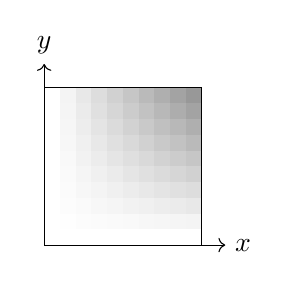
\begin{tikzpicture}[scale=2]
        \foreach \i in {0,1,...,9} \foreach \j in {0,1,...,9} {
            \pgfmathsetmacro{\d}{0.005*\i*\j}
            \fill[black,opacity=\d] (\i*0.1,\j*0.1) rectangle ({(\i+1)*0.1},{(\j+1)*0.1});
        }
        \draw (0,0) rectangle (1,1);
        \draw[->] (0,0)--(1.15,0) node[right]{$x$};
        \draw[->] (0,0)--(0,1.15) node[above]{$y$};
    \end{tikzpicture}
    \end{center}
    \item (Stewart \S15.4 \#7) Let $D$ be the triangle with vertices $(0,0)$, $(2,1)$, $(0,3)$ and density $\rho(x,y) = x+y$. Find the mass and the center of mass.
    \item Find the area of the region bounded by $y=x^2$ and $y=2x$ using a double integral.
    \item Find the centroid of the region bounded by $y=x$ and $y=x^2$.
    \item Find the mass of the lamina bounded by $y=\sqrt{x}$, $y=0$, $x=1$ with density $\rho(x,y)=x$.
\end{enumerate}

\subsubsection{Polar Coordinates}
\begin{enumerate}
    \item \dimtag{2D} (Stewart \S15.3 \#1--4) For each region shown below, decide whether polar or rectangular coordinates are more appropriate, and write $\iint_R f(x,y)\,dA$ as an iterated integral.
    \begin{center}
    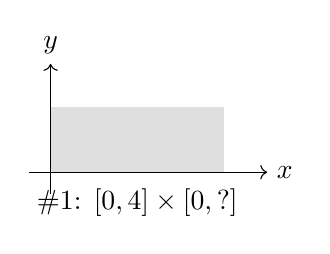
\begin{tikzpicture}[scale=0.55]
        \draw[->] (-0.5,0)--(5,0) node[right]{$x$}; \draw[->] (0,-0.5)--(0,2.5) node[above]{$y$};
        \fill[gray!25] (0,0) rectangle (4,1.5);
        \node at (2,-0.7) {\#1: $[0,4]\times[0,?]$};
    \end{tikzpicture}\quad
    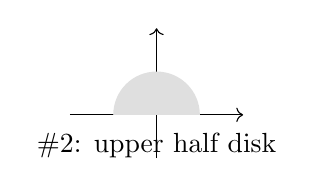
\begin{tikzpicture}[scale=0.55]
        \draw[->] (-2,0)--(2,0); \draw[->] (0,-1)--(0,2);
        \fill[gray!25] (0,0) -- (1,0) arc[start angle=0,end angle=180,radius=1] -- cycle;
        \node at (0,-0.7) {\#2: upper half disk};
    \end{tikzpicture}\quad
    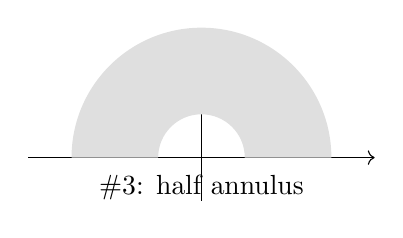
\begin{tikzpicture}[scale=0.55]
        \draw[->] (-4,0)--(4,0); \draw[->] (0,-1)--(0,2.5);
        \fill[gray!25] (-3,0) -- (-1,0) arc[start angle=180,end angle=0,radius=1] -- (3,0) arc[start angle=0,end angle=180,radius=3] -- cycle;
        \node at (0,-0.7) {\#3: half annulus};
    \end{tikzpicture}
    \end{center}
    \item (Stewart \S15.3 \#7) Sketch the region and evaluate $\displaystyle\int_{\pi/4}^{3\pi/4}\int_1^2 r\,dr\,d\theta$.
    \item (Stewart \S15.3 \#8) Sketch the region and evaluate $\displaystyle\int_0^{\pi/2}\int_0^{2\sin\theta} r\,dr\,d\theta$.
    \item (Stewart \S15.3 \#13) Evaluate $\iint_D e^{-(x^2+y^2)}\,dA$, where $D$ is the region bounded by the semicircle $x = \sqrt{4-y^2}$ and the $y$-axis.
    \item Evaluate $\iint_{D} e^{-(x^2 + y^2)} \, dA$, where $D$ is the region bounded by the semicircle $x = \sqrt{4 - y^2}$ and the $y$-axis.
    \item Use polar coordinates to find the volume of the solid bounded by the plane $z=0$ and the paraboloid $z = 1 - x^2 - y^2$.
    \item Setup and evaluate an integral in polar coordinates to find the area of one loop of the rose $r = \cos(3\theta)$.
    \item Evaluate $\int_{-1}^{1} \int_{0}^{\sqrt{1-x^2}} (x^2 + y^2)^{3/2} \, dy \, dx$ by converting to polar coordinates.
    \item  Find the area of the region that lies inside the cardioid $r = 1 + \cos \theta$ and outside the circle $r = 3\cos \theta$.
    \item Evaluate $\iint_D (x^2+y^2)\,dA$ where $D$ is the disk $x^2+y^2\le 4$.
    \item Find the area enclosed by one loop of $r=\sin 2\theta$.
    \item Convert to polar and evaluate $\displaystyle\int_0^2\!\int_0^{\sqrt{4-x^2}} \sqrt{x^2+y^2}\,dy\,dx$.
    \item Find the area inside the cardioid $r=1+\cos\theta$.
\end{enumerate}

\subsubsection{Triple Integrals in Rectangular and Cylindrical}
\begin{enumerate}
    \item \dimtag{3D} Evaluate $\iiint_{E} xyz \, dV$, where $E$ is the rectangular box $[0, 1] \times [0, 2] \times [0, 3]$.
    \item (Stewart \S15.6 \#9) Let $E$ be the solid bounded above by $z = 1 - x^2$, the plane $y = 0$, and the planes $x + z = 2$ and $x = \sqrt{y}$ (see figure). For $f(x,y,z) = x$, do two things. (a) Express $\iiint_E f\,dV$ as an iterated integral. (b) Evaluate it.
    \begin{center}
    \begin{tikzpicture}[scale=0.8, x={(1cm,0cm)}, y={(-0.5cm,-0.4cm)}, z={(0cm,1cm)}]
        \draw[->] (0,0,0)--(3,0,0) node[right]{$x$};
        \draw[->] (0,0,0)--(0,3,0) node[below right]{$y$};
        \draw[->] (0,0,0)--(0,0,2.5) node[above]{$z$};
        \fill[gray!30,opacity=0.6] (0,0,0) -- (1,0,0) -- (1,1,0) -- (0,0,0);
        \draw plot[smooth,samples=20,domain=0:1] (\x, {\x*\x}, 0);
        \draw plot[smooth,samples=20,domain=0:1] (\x, 0, {1-\x*\x});
        \node at (0.7,0.3,0.7) {\footnotesize $E$};
        \node at (0.5,0,1) {\footnotesize $z=1-x^2$};
    \end{tikzpicture}
    \end{center}
    \item (Stewart \S15.6 \#10) For $f(x,y,z) = xy$ and $E$ bounded by $y + z = 2$, $z = 4 - y^2$, $y = x$, $x = 0$, write $\iiint_E f\,dV$ as an iterated integral and evaluate it.
    \item Find the volume of the tetrahedron bounded by the planes $x=0, y=0, z=0$ and $x + y + z = 1$.
    \item (Stewart \S15.6 \#23, adapted) Evaluate $\iiint_T y^2\,dV$ where $T$ is the solid tetrahedron with vertices $(0,0,0)$, $(2,0,0)$, $(0,2,0)$, $(0,0,2)$.
    \item (Stewart \S15.6 \#32, adapted) Sketch the solid whose volume is given by
    \[ \int_0^2 \int_0^{2-y}\int_0^{4 - y^2}\, dx\, dz\, dy. \]
    \item Use cylindrical coordinates to find the volume of the solid that lies within the cylinder $x^2 + y^2 = 1$, below the plane $z = 4$, and above the paraboloid $z = 1 - x^2 - y^2$.
    \item (Stewart \S15.7 \#11) Sketch the solid described by $r^2 \leq z \leq 8 - r^2$.
    \item (Stewart \S15.7 \#12) Sketch the solid described by $0 \leq \theta \leq \pi/2,\ r \leq z \leq 2$.
    \item (Stewart \S15.7 \#18) Sketch the solid whose volume is given by
    \[ \int_0^2 \int_0^{2\pi}\int_0^{r} r\,dz\,d\theta\,dr, \]
    and evaluate the integral.
    \item (Stewart \S15.7 \#19) Use cylindrical coordinates to evaluate $\iiint_E \sqrt{x^2+y^2}\,dV$ where $E$ is the region inside the cylinder $x^2 + y^2 = 16$ and between $z = -5$ and $z = 4$.
    \item (Stewart \S15.7 \#20) Evaluate $\iiint_E z\, dV$ where $E$ is enclosed by the paraboloid $z = x^2 + y^2$ and the plane $z = 4$.
    \item Evaluate $\iiint_{E} (x^2 + y^2) \, dV$, where $E$ is the region bounded by the cylinder $x^2 + y^2 = 4$ and the planes $z = -1$ and $z = 2$.
    \item (Stewart \S15.7 \#26) Find the volume of the solid that lies between the paraboloid $z = x^2 + y^2$ and the sphere $x^2 + y^2 + z^2 = 2$.
    \item (Stewart \S15.7 \#32) Evaluate by changing to cylindrical coordinates.
    \[ \int_0^2 \int_0^{\sqrt{4-y^2}}\int_{-2}^{2} xz\, dz\,dx\,dy. \]
    \item  Find the volume of the solid bounded by the cylinders $x^2+y^2=1$ and $x^2+z^2=1$ (the Steinmetz solid)
    \item Find the volume of the solid bounded below by $z=x^2+y^2$ and above by $z=8-x^2-y^2$.
    \item Find the mass of the cylinder $x^2+y^2\le 1$, $0\le z\le 2$, with density $\rho=z$.
    \item Evaluate $\iiint_E \sqrt{x^2+y^2}\,dV$ inside the cylinder $x^2+y^2\le 4$ between $z=0$ and $z=3$.
\end{enumerate}

\subsubsection{Triple Integrals in Spherical Coordinates}
\begin{enumerate}
    \item \dimtag{3D} Evaluate $\iiint_{B} e^{(x^2+y^2+z^2)^{3/2}} \, dV$, where $B$ is the unit ball.
    \item (Stewart \S15.8 \#19) Set up the triple integral of an arbitrary continuous function $f(x,y,z)$ in cylindrical or spherical coordinates over the solid shown below, a cone of half-angle $\pi/3$ inside a sphere of radius $3$ centered at the origin, the ice cream cone.
    \begin{center}
    \begin{tikzpicture}[scale=0.8, x={(1cm,0cm)}, y={(-0.5cm,-0.4cm)}, z={(0cm,1cm)}]
        \draw[->] (0,0,0)--(3,0,0) node[right]{$x$};
        \draw[->] (0,0,0)--(0,3,0) node[below right]{$y$};
        \draw[->] (0,0,0)--(0,0,3.5) node[above]{$z$};
        \draw[blue!70] (0,0,0) -- (1.5,0,2.6);
        \draw[blue!70] (0,0,0) -- (-1.5,0,2.6);
        \draw[blue!70] (0,1.5,2.6) arc[start angle=90,end angle=-90,x radius=1.5,y radius=0.4];
        \draw[blue!70,dashed] (0,-1.5,2.6) arc[start angle=270,end angle=90,x radius=1.5,y radius=0.4];
        \draw[red!70] (0,0,3) arc[start angle=90,end angle=270,radius=3];
        \node at (1.5,0,1.5) {\small $E$};
    \end{tikzpicture}
    \end{center}
    \item (Stewart \S15.8 \#24) Evaluate $\iiint_E y^2 z^2\, dV$, where $E$ lies above the cone $\phi = \pi/3$ and below the sphere $\rho = 1$.
    \item Find the volume of the solid that lies above the cone $z = \sqrt{x^2 + y^2}$ and below the sphere $x^2 + y^2 + z^2 = z$.
    \item (Stewart \S15.8 \#27) Evaluate $\iiint_E x\,e^{x^2 + y^2 + z^2}\, dV$, where $E$ is the portion of the unit ball $x^2+y^2+z^2 \leq 1$ that lies in the first octant.
    \item (Stewart \S15.8 \#30) Find the average distance from a point in a ball of radius $a$ to its center.
    \item Set up the integral to find the mass of a spherical shell $1 \le \rho \le 2$ if the density is $\delta(\rho, \phi, \theta) = \rho$.
    \item Find the volume of the ``ice cream cone'' solid cut from the sphere $\rho \le a$ by the cone $\phi = \alpha$.
    \item Let $E$ be the region in the first octant ($x \geq 0, y \geq 0, z \geq 0$) between the spheres of radius 1 and radius 3 centered at the origin.
    \begin{enumerate}
        \item Write the bounds for $\rho$, $\phi$, and $\theta$ in spherical coordinates.
        \item Evaluate $\iiint_E z \, dV$.
    \end{enumerate}
    \item Use spherical coordinates to evaluate $\iiint_E (x^2 + y^2 + z^2) \, dV$ where $E$ is the solid in the first octant bounded by the sphere $x^2+y^2+z^2 = 9$ and the coordinate planes.
    \item (Stewart \S15.8 \#44) Evaluate by changing to spherical coordinates.
    \[ \int_{-a}^{a}\int_{-\sqrt{a^2-y^2}}^{\sqrt{a^2-y^2}}\int_{-\sqrt{a^2-x^2-y^2}}^{\sqrt{a^2-x^2-y^2}} (x^2 z + y^2 z + z^3)\, dz\,dx\,dy. \]
    \item Find the volume of a ball of radius $a$ using spherical coordinates.
    \item Evaluate $\iiint_B (x^2+y^2+z^2)\,dV$ over the ball $\rho\le 2$.
    \item Find the mass of the ball $\rho\le 1$ with density $\delta=\rho$.
    \item Find the volume of the solid above the cone $\phi=\pi/4$ and inside the sphere $\rho=2$.
\end{enumerate}

\subsubsection{Coordinate Transformations (Jacobians)}
\begin{enumerate}
    \item \dimtag{2D} Evaluate $\iint_R (x+y) e^{x-y} \, dA$ where $R$ is the diamond bounded by $x+y=1, x+y=3, x-y=-1, x-y=1$ using $u=x+y$ and $v=x-y$.
    \item Use the transformation $x=au, y=bv$ to find the area of the ellipse $\frac{x^2}{a^2} + \frac{y^2}{b^2} = 1$.
    \item Evaluate $\iint_R \cos\left( \frac{y-x}{y+x} \right) \, dA$ where $R$ is the triangle with vertices $(0,0), (1,0), (0,1)$.
    \item Compute the Jacobian $\dfrac{\partial(x,y)}{\partial(u,v)}$ for $x=u^2-v^2$, $y=2uv$.
    \item Confirm that the polar change of variables gives $\dfrac{\partial(x,y)}{\partial(r,\theta)}=r$.
\end{enumerate}

\subsection{Vector Calculus (Part A)}

\subsubsection{Vector Fields}
\begin{enumerate}
    \item \dimtag{2D} The dome's downhill flow is its gradient field $\vec F = \nabla f = \langle -2x, -2y\rangle$, where $f = 1 - x^2 - y^2$. Draw $\vec F$ at $(\pm1,0)$, $(0,\pm1)$, and $(\pm1,\pm1)$, each arrow scaled down by half. Which way does every arrow point, and how does that match water running off the dome?
    \item \dimtag{2D} On the same axes sketch a few level curves of $f$ (circles) and check that each arrow of $\vec F$ crosses its circle at a right angle, longest where the circles crowd together. This is the gradient picture from the last chapter, now drawn as a field.
    \item \dimtag{2D} Contrast the swirl $\vec G = \langle -y, x\rangle$. Draw it at the same points. Walk a small loop and watch the height fail to return, then say in one line why no surface has $\vec G$ as its gradient.
    \item \dimtag{2D} Sketch the vector field $\vec{F}(x,y) = \langle -y, x \rangle$.
    \item (Stewart \S16.1 \#2) Sketch the vector field $\vec F(x,y) = 2\,\ihat - \jhat$.
    \item (Stewart \S16.1 \#4) Sketch $\vec F(x,y) = x\,\ihat + \tfrac{1}{2}y\,\jhat$.
    \item (Stewart \S16.1 \#8) Sketch $\vec F(x,y) = \dfrac{y\,\ihat - x\,\jhat}{\sqrt{x^2+y^2}}$.
    \item (Stewart \S16.1 \#10) Sketch the 3D vector field $\vec F(x,y,z) = z\,\ihat$.
    \item (Stewart \S16.1 \#13--18, matching) Each plot below sketches a planar vector field. Match each formula to a plot and explain.
    \begin{enumerate}
        \item $\vec F(x,y) = \langle x, -y\rangle$
        \item $\vec F(x,y) = \langle y,\ y+2\rangle$
        \item $\vec F(x,y) = \langle y,\ -x\rangle$
        \item $\vec F(x,y) = \langle \sin y,\ \cos x\rangle$
    \end{enumerate}
    \item (Stewart \S16.1 \#19--22, matching) Match each 3D vector field to its plot.
    \begin{enumerate}
        \item $\vec F = \ihat + 2\jhat + 3\khat$
        \item $\vec F = \ihat + 2\jhat + z\,\khat$
        \item $\vec F = x\,\ihat + y\,\jhat + 3\khat$
        \item $\vec F = x\,\ihat + y\,\jhat + z\,\khat$
    \end{enumerate}
    \item (Stewart \S16.1 \#31--34, matching) Match each function $f$ to a plot of its gradient field $\nabla f$.
    \begin{enumerate}
        \item $f(x,y) = x^2 + y^2$
        \item $f(x,y) = x(x+y)$
        \item $f(x,y) = (x+y)^2$
        \item $f(x,y) = \sin\sqrt{x^2+y^2}$
    \end{enumerate}
    \item Sketch the vector fields $\vec F(x,y)=\langle x,y\rangle$ and $\vec F(x,y)=\langle x,-y\rangle$.
    \item Find the gradient field $\nabla f$ for $f(x,y)=x^2+y^2$ and for $f(x,y)=x^2-y^2$, and sketch each.
    \item Determine whether $\vec F=\langle y,x\rangle$ is a gradient field, and if so find a function $f$ with $\nabla f=\vec F$.
\end{enumerate}

\subsubsection{Line Integrals (Scalar and Vector)}
\begin{enumerate}
    \item \dimtag{1D in 3D} Evaluate the line integral $\int_C y\,ds$, where $C$ is the right half of the circle $x^2 + y^2 = 1$ from $(0,-1)$ to $(0,1)$.
    \item (Stewart \S16.2 \#1) Evaluate $\int_C y\,ds$, where $C$ is given by $x = t^3,\ y = 2t,\ 0 \leq t \leq 3/2$.
    \item (Stewart \S16.2 \#3) Evaluate $\int_C xy^4\,ds$ where $C$ is the right half of the circle $x^2 + y^2 = 16$.
    \item (Stewart \S16.2 \#9) Evaluate $\int_C x^2 y\,ds$ where $C$ is given by $x = \cos t,\ y = \sin t,\ z = t,\ 0 \leq t \leq \pi/2$.
    \item (Stewart \S16.2 \#11) Evaluate $\int_C x\,e^{yz}\,ds$ where $C$ is the line segment from $(0,0,0)$ to $(1,2,3)$.
    \item (Stewart \S16.2 \#12) Evaluate $\int_C (x^2 + y^2 + z^2)\, ds$ where $C$ is given by $x=t,\ y=\cos 2t,\ z=\sin 2t,\ 0\leq t \leq 2\pi$.
    \item Find the work done by the force field $\vec{F}(x,y) = \langle x^2, -xy \rangle$ along the quarter-circle $\vec{r}(t) = \langle \cos t, \sin t \rangle$ for $0 \leq t \leq \pi/2$.
    \item (Stewart \S16.2 \#5) Evaluate $\int_C (x^2 y + \sin x)\,dy$ where $C$ is the arc of the parabola $y = x^2$ from $(0,0)$ to $(\pi,\pi^2)$.
    \item (Stewart \S16.2 \#8) Evaluate $\int_C x^2\,dx + y^2\,dy$ where $C$ is the arc of $x^2 + y^2 = 4$ from $(-1,1)$ to $(2,0)$ traversed through $(0,2)$ (see figure).
    \begin{center}
    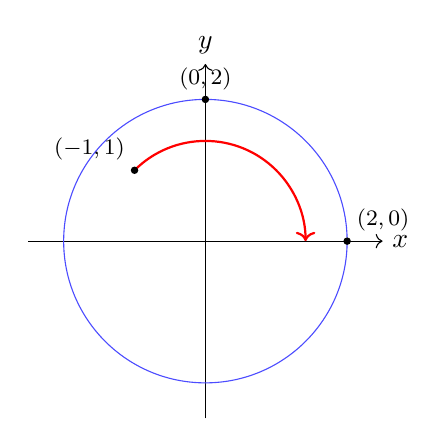
\begin{tikzpicture}[scale=0.9]
        \draw[->] (-2.5,0)--(2.5,0) node[right]{$x$};
        \draw[->] (0,-2.5)--(0,2.5) node[above]{$y$};
        \draw[blue!70] (0,0) circle (2);
        \draw[red,thick,->] (-1,1) arc[start angle=135, end angle=0, radius=1.414];
        \fill (-1,1) circle (1.5pt) node[above left]{\footnotesize $(-1,1)$};
        \fill (0,2) circle (1.5pt) node[above]{\footnotesize $(0,2)$};
        \fill (2,0) circle (1.5pt) node[above right]{\footnotesize $(2,0)$};
    \end{tikzpicture}
    \end{center}
    \item Evaluate $\int_{C} \vec{F} \cdot d\vec{r}$, where $\vec{F} = \langle z, x, y \rangle$ and $C$ is the helix $\vec{r}(t) = \langle \cos t, \sin t, t \rangle$ for $0 \leq t \leq \pi$.
    \item (Stewart \S16.2 \#15) Evaluate $\int_C z\,dx + xy\,dy + y^2\,dz$ where $C$ is given by $x = \sin t,\ y = \cos t,\ z = \tan t$, $-\pi/4 \leq t \leq \pi/4$.
    \item Evaluate the scalar line integral $\displaystyle\int_C (x + yz) \, ds$ where $C$ is the twisted cubic $\vec{r}(t) = \langle t, t^2, t^3 \rangle$ for $0 \leq t \leq 1$.
    \item  Evaluate $\int_C (x^2 + y^2) \, ds$ where $C$ is the ``bent'' path from $(0,0,0)$ to $(1,2,3)$ consisting of three straight line segments parallel to the axes.
    \item Find the work done by $\vec{F} = \langle \sin x, \cos y, xz \rangle$ along the curve $\vec{r}(t) = \langle t^3, -t^2, t \rangle$ from $t=0$ to $t=1$.
    \item (Stewart \S16.2 \#21) Evaluate $\int_C \vec F\cdot d\vec r$ for $\vec F(x,y) = xy^2\,\ihat - x^2\,\jhat$ where $\vec r(t) = t^3\,\ihat + t^2\,\jhat$, $0\leq t \leq 1$.
    \item (Stewart \S16.2 \#19) The vector field $\vec F$ is shown below.
    \begin{center}
    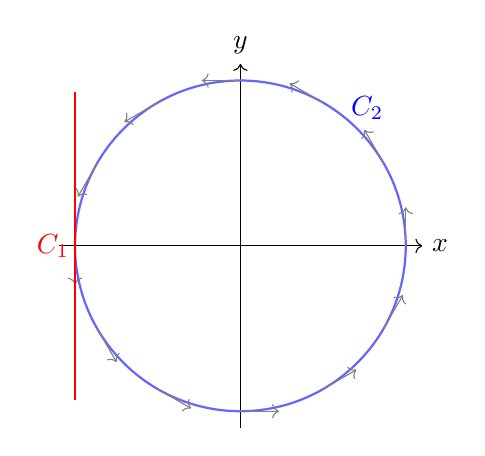
\begin{tikzpicture}[scale=0.7]
        \draw[->] (-3.3,0)--(3.3,0) node[right]{$x$};
        \draw[->] (0,-3.3)--(0,3.3) node[above]{$y$};
        \draw[blue!60,thick] (0,0) circle (3);
        \foreach \a in {0,30,...,330}{
            \draw[->,gray] ({3*cos(\a)},{3*sin(\a)}) -- ({3*cos(\a) - 0.7*sin(\a)},{3*sin(\a) + 0.7*cos(\a)});
        }
        \draw[red,thick] (-3,-2.8)--(-3,2.8);
        \node[red] at (-3.4,0) {$C_1$};
        \node[blue] at (2.3,2.5) {$C_2$};
    \end{tikzpicture}
    \end{center}
    (a) If $C_1$ is the vertical line segment from $(-3,-3)$ to $(-3,3)$, decide if $\int_{C_1}\vec F\cdot d\vec r$ is positive, negative, or zero.
    (b) If $C_2$ is the counterclockwise circle of radius $3$ centered at the origin, decide the sign of $\int_{C_2}\vec F\cdot d\vec r$.
    \item (Stewart \S16.2 \#20) The figure below shows another field $\vec F$ and two curves $C_1, C_2$. Are the line integrals positive, negative, or zero? Explain.
    \begin{center}
    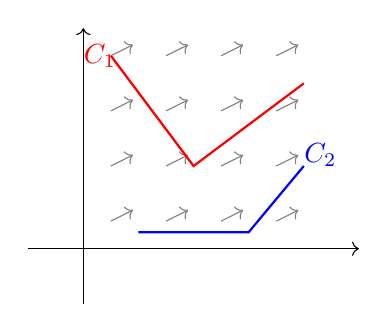
\begin{tikzpicture}[scale=0.7]
        \draw[->] (-1,0)--(5,0); \draw[->] (0,-1)--(0,4);
        \foreach \x in {0.5,1.5,2.5,3.5} \foreach \y in {0.5,1.5,2.5,3.5}
            \draw[->,gray] (\x,\y) -- ({\x+0.4},{\y+0.2});
        \draw[red,thick] (0.5,3.5)--(2,1.5)--(4,3);
        \node[red] at (0.3,3.5) {$C_1$};
        \draw[blue,thick] (1,0.3)--(3,0.3)--(4,1.5);
        \node[blue] at (4.3,1.7) {$C_2$};
    \end{tikzpicture}
    \end{center}
    \item Evaluate $\int_C xy\,ds$ where $C$ is the segment from $(0,0)$ to $(1,2)$.
    \item Evaluate $\int_C y\,dx+x\,dy$ along $\vec r(t)=\langle t,\ t^2\rangle$, $0\le t\le 1$.
    \item Evaluate $\int_C \vec F\cdot d\vec r$ for $\vec F=\langle x^2,\ xy\rangle$ along the unit circle traversed counterclockwise.
    \item Find the work done by $\vec F=\langle x+y,\ x-y\rangle$ along the segment from $(0,0)$ to $(2,3)$.
\end{enumerate}

\subsubsection{Conservative Fields and Potential Functions}
\begin{enumerate}
    \item \dimtag{2D} The dome height $f = 1 - x^2 - y^2$ is a potential for its gradient field $\vec F = \langle -2x, -2y\rangle$, so $\vec F$ is conservative. Argue the work along any curve from $(1,0)$ to $(0,0)$ is just the height gained, $f(0,0) - f(1,0)$, whatever the path. Sketch two different paths and confirm they agree.
    \item \dimtag{2D} (Stewart \S16.3 \#1) The figure shows a curve $C$ and a contour map of a function $f$ whose gradient is continuous. The curve $C$ starts on the level $f = 10$ and ends on the level $f = 60$. Use the picture to find $\int_C \nabla f\cdot d\vec r$.
    \begin{center}
    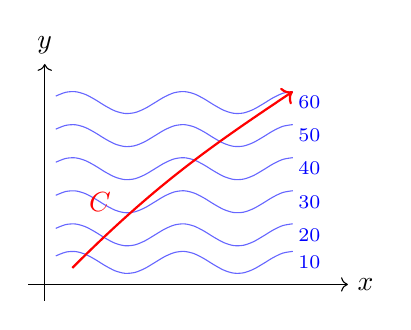
\begin{tikzpicture}[scale=0.7]
        \draw[->] (-0.3,0)--(5.5,0) node[right]{$x$};
        \draw[->] (0,-0.3)--(0,4) node[above]{$y$};
        \foreach \k/\h in {10/0.4, 20/0.9, 30/1.5, 40/2.1, 50/2.7, 60/3.3}{
            \draw[blue!60] plot[smooth,samples=25,domain=0.2:4.5] (\x, {\h + 0.2*sin(180*\x)});
            \node[blue,font=\scriptsize] at (4.8,\h) {\k};
        }
        \draw[red,thick,->] (0.5,0.3) .. controls (2,1.8) and (3,2.5) .. (4.5,3.5);
        \node[red] at (1,1.5) {$C$};
    \end{tikzpicture}
    \end{center}
    \item (Stewart \S16.3 \#2) A table of values of a function $f$ with continuous gradient is given (selected values shown). Find $\int_C \nabla f\cdot d\vec r$, where $C$ has parametric equations $x = t^2 + 1,\ y = t^3 + t$, $0 \leq t \leq 1$.
    \begin{center}\begin{tabular}{c|ccc}
        $x \backslash y$ & 0 & 1 & 2 \\\hline
        0 & 1 & 6 & 4 \\
        1 & 3 & 5 & 7 \\
        2 & 8 & 2 & 9
    \end{tabular}\end{center}
    \item Determine whether $\vec{F}(x,y) = \langle 3 + 2xy, x^2 - 3y^2 \rangle$ is conservative. If it is, find a potential function $f$.
    \item (Stewart \S16.3 \#4) Determine whether $\vec F(x,y) = (y-2x)\,\ihat + 2xy\,\jhat$ is conservative, and if so find $f$ with $\vec F = \nabla f$.
    \item (Stewart \S16.3 \#8) Determine whether $\vec F(x,y) = (2xy + y^{-2})\,\ihat + (x^2 - 2xy^{-3})\,\jhat$ (with $y > 0$) is conservative.
    \item Show that $\vec{F}(x,y,z) = \langle yz, xz, xy \rangle$ is conservative and find $f$ such that $\nabla f = \vec{F}$.
    \item Use the Fundamental Theorem for Line Integrals to evaluate $\int_{C} \nabla f \cdot d\vec{r}$ where $f(x,y) = \sin(x) + x^2y$ and $C$ is any path from $(0,0)$ to $(\pi, 2)$.
    \item (Stewart \S16.3 \#11) The figure shows the vector field $\vec F(x,y) = \langle 2xy,\ x^2\rangle$ and three curves $C_1, C_2, C_3$ that each start at $(1,2)$ and end at $(3,2)$.
    \begin{center}
    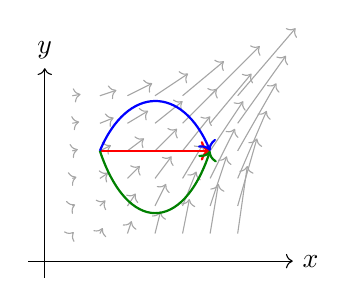
\begin{tikzpicture}[scale=0.7]
        \draw[->] (-0.3,0)--(4.5,0) node[right]{$x$};
        \draw[->] (0,-0.3)--(0,3.5) node[above]{$y$};
        \foreach \x in {0.5,1,1.5,2,2.5,3,3.5} \foreach \y in {0.5,1,1.5,2,2.5,3} {
            \pgfmathsetmacro{\u}{0.3*\x*\y/3}
            \pgfmathsetmacro{\v}{0.3*\x*\x/3}
            \draw[->,gray!70] (\x,\y) -- ({\x+\u},{\y+\v});
        }
        \draw[red,thick,->] (1,2) -- (3,2);
        \draw[blue,thick,->] (1,2) .. controls (1.5,3.2) and (2.5,3.2) .. (3,2);
        \draw[green!50!black,thick,->] (1,2) .. controls (1.5,0.5) and (2.5,0.5) .. (3,2);
    \end{tikzpicture}
    \end{center}
    (a) Explain why $\int_{C_i}\vec F\cdot d\vec r$ has the same value for all three. (b) Compute this common value.
    \item (Stewart \S16.3 \#12) Evaluate $\int_C \vec F\cdot d\vec r$ for $\vec F(x,y) = 2xy\,\ihat + (x^2 + \sin y)\,\jhat$ along (a) any path from $(0,0)$ to $(2, \pi/2)$ and (b) any path from $(0,0)$ to $(1,1)$ along $y = \sin(\pi x/2)$.
    \item (Stewart \S16.3 \#13) Let $\vec F(x,y) = (3x^2 + y^2)\,\ihat + 2xy\,\jhat$ and let $C$ be the upper half of the circle of radius $2$ centered at origin from $(-2,0)$ to $(2,0)$ via the lower semicircle (see figure).
    (a) Evaluate $\int_C \vec F\cdot d\vec r$ directly. (b) Show $\vec F$ is conservative and find $f$. (c) Re-evaluate using the FTC. (d) Replace $C$ by a simpler path with the same endpoints and re-evaluate.
    \item (Stewart \S16.3 \#14) Let $\vec F(x,y) = \langle \sin y + e^x,\ x\cos y\rangle$ and $C$ given by $x=t$, $y=t(3-t)$, $0\leq t\leq 3$.
    (a) Show $\vec F$ is conservative, find $f$. (b) Use FTC. (c) Replace $C$ by a line segment with the same endpoints, then re-evaluate.
    \item Find the work done by the field $\vec{F} = \langle 2xe^y, x^2e^y + \cos y \rangle$ along the path $y = \sin x$ from $(0,0)$ to $(\pi, 0)$.
    \item (Stewart \S16.3 \#18) Find $f$ with $\nabla f = \vec F$ for $\vec F = (3 + 2xy^2)\,\ihat + 2x^2 y\,\jhat$, and use it to evaluate $\int_C \vec F\cdot d\vec r$ where $C$ is the arc of $y = 1/x$ from $(1,1)$ to $(4, 1/4)$.
    \item (Stewart \S16.3 \#20) Find $f$ such that $\vec F = \nabla f$ for $\vec F = (1+xy)e^{xy}\,\ihat + x^2 e^{xy}\,\jhat$, then evaluate $\int_C \vec F\cdot d\vec r$ on $\vec r(t) = \cos t\,\ihat + 2\sin t\,\jhat$, $0\leq t\leq \pi/2$.
    \item Determine if $\vec{F} = \langle e^y, xe^y + e^z, ye^z \rangle$ is conservative. If so, find $f$.
    \item Evaluate $\int_C \vec{F} \cdot d\vec{r}$ for $\vec{F} = \langle e^y, xe^y + e^z, ye^z \rangle$ along any path from $(0,0,0)$ to $(1,1,1)$.
    \item Show $\vec F=\langle 2xy,\ x^2+3y^2\rangle$ is conservative and find a potential $f$.
    \item Using the potential from the previous problem, evaluate $\int_C \vec F\cdot d\vec r$ from $(0,0)$ to $(1,2)$.
    \item Determine whether $\vec F=\langle y^2,\ 2xy+e^{3z},\ 3y e^{3z}\rangle$ is conservative, and if so find a potential.
    \item Is $\vec F=\dfrac{\langle -y,\ x\rangle}{x^2+y^2}$ conservative on the plane with the origin removed? Test $P_y=Q_x$ and explain the role of the hole.
\end{enumerate}

\subsubsection{Green's Theorem}
\begin{enumerate}
    \item \dimtag{2D} (Stewart \S16.4 \#1) Evaluate $\oint_C y^2\,dx + x^2 y\,dy$ where $C$ is the rectangle with vertices $(0,0),\ (5,0),\ (5,4),\ (0,4)$, by two methods, first directly and then using Green's Theorem.
    \item (Stewart \S16.4 \#2) Evaluate $\oint_C y\,dx - x\,dy$ where $C$ is the circle of radius $4$ centered at the origin, by (a) direct computation and (b) Green's Theorem.
    \item Use Green's Theorem to evaluate $\oint_{C} (y^2 \, dx + 3xy \, dy)$, where $C$ is the boundary of the upper semi-annulus $1 \leq x^2 + y^2 \leq 4, y \geq 0$.
    \item (Stewart \S16.4 \#6) Use Green's Theorem to evaluate $\oint_C \ln(xy)\,dx + (y/x)\,dy$ where $C$ is the rectangle with vertices $(1,1),\ (1,4),\ (2,4),\ (2,1)$.
    \item (Stewart \S16.4 \#8) Use Green's Theorem on $\oint_C (x^2 + y^2)\,dx + (x^2 - y^2)\,dy$ where $C$ is the triangle with vertices $(0,0),\ (2,1),\ (0,1)$.
    \item Use Green's Theorem to find the area of the ellipse $\frac{x^2}{a^2} + \frac{y^2}{b^2} = 1$ using the formula $A = \frac{1}{2} \oint_{C} (x \, dy - y \, dx)$.
    \item Evaluate $\oint_C (xy + y^2)dx + (x^2)dy$ where $C$ is the boundary of the region between $y=x$ and $y=x^2$.
    \item (Stewart \S16.4 \#12) Use Green's Theorem to evaluate $\oint_C (1 - y^3)\,dx + (x^3 + e^{y^2})\,dy$ where $C$ is the boundary of the region between $x^2 + y^2 = 4$ and $x^2 + y^2 = 9$ (positively oriented).
    \item (Stewart \S16.4 \#14) Use Green's Theorem to compute $\oint_C (x^{2/3} + y^3)\,dx + (y^{4/3} - x^3)\,dy$ where $C$ is the boundary of the region bounded by $x = y^2$ and $x = 4$, traversed positively (see figure).
    \begin{center}
    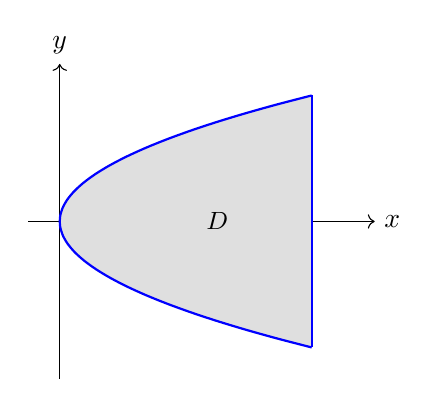
\begin{tikzpicture}[scale=0.8]
        \draw[->] (-0.5,0)--(5,0) node[right]{$x$};
        \draw[->] (0,-2.5)--(0,2.5) node[above]{$y$};
        \fill[gray!25] plot[smooth,samples=30,domain=-2:2] ({\x*\x},\x) -- (4,2) -- (4,-2) -- cycle;
        \draw[blue,thick] plot[smooth,samples=30,domain=-2:2] ({\x*\x},\x);
        \draw[blue,thick] (4,-2)--(4,2);
        \node at (2.5,0) {\small $D$};
    \end{tikzpicture}
    \end{center}
    \item Use Green's Theorem to evaluate $\oint_C \vec{F} \cdot d\vec{r}$ where $\vec{F} = \langle e^x - y^3, \cos y + x^3 \rangle$ and $C$ is the unit circle.
    \item Use Green's Theorem to find the work done by $\vec{F} = \langle y + e^{\sqrt{x}}, 2x + \cos(y^2) \rangle$ on a particle moving once counterclockwise around the unit circle.
    \item Evaluate $\oint_C \frac{-y}{x^2+y^2} \, dx + \frac{x}{x^2+y^2} \, dy$ where $C$ is a circle of radius 1 centered at $(0,0)$. Why does Green's Theorem require care here?
    \item Use Green's Theorem to evaluate $\oint_C (y^2\,dx+x^2\,dy)$ around the unit square, counterclockwise.
    \item Use $\tfrac12\oint_C (x\,dy-y\,dx)$ to find the area enclosed by the ellipse $x=a\cos t$, $y=b\sin t$.
    \item Use Green's Theorem to evaluate $\oint_C (xy\,dx+x^2\,dy)$ around the triangle $(0,0),(1,0),(1,1)$.
\end{enumerate}

\newpage
\center{\section{Pre-Final Material}}

\subsection{Vector Calculus (Part B)}

\subsubsection{Curl and Divergence}
\begin{enumerate}
    \item \dimtag{2D} Return to the dome's two fields. For the downhill gradient field $\vec F = \langle -2x, -2y\rangle$ compute $\operatorname{div}\vec F$ and $\operatorname{curl}\vec F$, and read the signs as a sink at the peak with no spin. For the swirl $\vec G = \langle -y, x\rangle$ compute both and read a pure spin with no net outflow. Sketch a tiny paddle wheel in each field at $(1,0)$.
    \item \dimtag{3D} (Stewart \S16.5 \#1) Find (a) the curl and (b) the divergence of $\vec F(x,y,z) = xy^2 z^2\,\ihat + x^2 y z^2\,\jhat + x^2 y^2 z\,\khat$.
    \item Find the curl and divergence of the vector field $\vec{F}(x,y,z) = \langle xz, xyz, -y^2 \rangle$.
    \item (Stewart \S16.5 \#9--12, figure-based) For each planar vector field shown, independent of $z$ with zero $z$-component, determine the following at the marked point $P$. (a) Is $\operatorname{div}\vec F$ positive, negative, or zero? (b) Is $\operatorname{curl}\vec F$ nonzero, and if so does it point in $+\khat$ or $-\khat$ at $P$?
    \begin{center}
    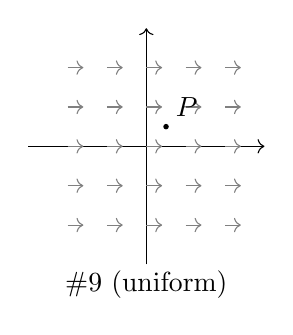
\begin{tikzpicture}[scale=0.5]
        \draw[->] (-3,0)--(3,0); \draw[->] (0,-3)--(0,3);
        \foreach \x in {-2,-1,0,1,2} \foreach \y in {-2,-1,0,1,2}
            \draw[->,gray] (\x,\y)--(\x+0.4,\y+0.0);
        \fill (0.5,0.5) circle (2pt) node[above right]{$P$};
        \node at (0,-3.5) {\#9 (uniform)};
    \end{tikzpicture}\quad
    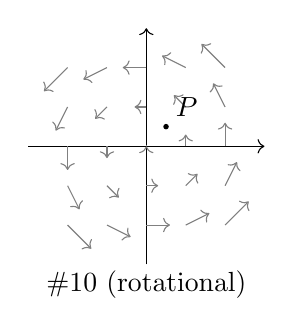
\begin{tikzpicture}[scale=0.5]
        \draw[->] (-3,0)--(3,0); \draw[->] (0,-3)--(0,3);
        \foreach \x in {-2,-1,0,1,2} \foreach \y in {-2,-1,0,1,2}{
            \pgfmathsetmacro{\u}{-0.3*\y} \pgfmathsetmacro{\v}{0.3*\x}
            \draw[->,gray] (\x,\y)--({\x+\u},{\y+\v});
        }
        \fill (0.5,0.5) circle (2pt) node[above right]{$P$};
        \node at (0,-3.5) {\#10 (rotational)};
    \end{tikzpicture}\quad
    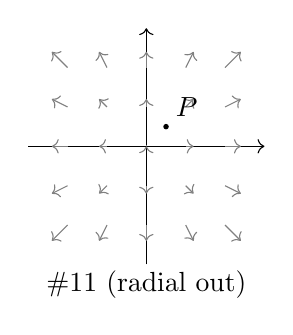
\begin{tikzpicture}[scale=0.5]
        \draw[->] (-3,0)--(3,0); \draw[->] (0,-3)--(0,3);
        \foreach \x in {-2,-1,0,1,2} \foreach \y in {-2,-1,0,1,2}{
            \pgfmathsetmacro{\u}{0.2*\x} \pgfmathsetmacro{\v}{0.2*\y}
            \draw[->,gray] (\x,\y)--({\x+\u},{\y+\v});
        }
        \fill (0.5,0.5) circle (2pt) node[above right]{$P$};
        \node at (0,-3.5) {\#11 (radial out)};
    \end{tikzpicture}\quad
    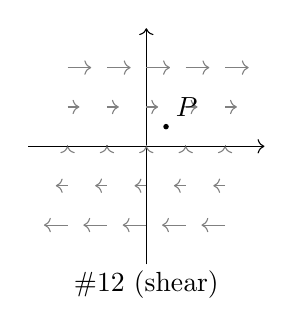
\begin{tikzpicture}[scale=0.5]
        \draw[->] (-3,0)--(3,0); \draw[->] (0,-3)--(0,3);
        \foreach \x in {-2,-1,0,1,2} \foreach \y in {-2,-1,0,1,2}{
            \pgfmathsetmacro{\u}{0.3*\y}
            \draw[->,gray] (\x,\y)--({\x+\u},\y);
        }
        \fill (0.5,0.5) circle (2pt) node[above right]{$P$};
        \node at (0,-3.5) {\#12 (shear)};
    \end{tikzpicture}
    \end{center}
    \item (Stewart \S16.5 \#13) (a) Verify Formula 3 (i.e.\ $\operatorname{curl}(\nabla f) = \vec 0$) for $f(x,y,z) = \sin(xyz)$. (b) Verify Formula 11 (i.e.\ $\operatorname{div}(\operatorname{curl}\vec F) = 0$) for $\vec F = xyz^2\,\ihat + x^2 y z^3\,\jhat + y^2\,\khat$.
    \item (Stewart \S16.5 \#14) Let $f$ be a scalar field and $\vec F$ a vector field. State whether each expression is meaningful, and if so say whether it is a scalar field or a vector field.
    (a) $\operatorname{curl} f$,\quad (b) $\operatorname{grad} f$,\quad (c) $\operatorname{div}\vec F$,\quad (d) $\operatorname{curl}(\operatorname{grad} f)$,\quad (e) $\operatorname{grad}\vec F$,\quad (f) $\operatorname{grad}(\operatorname{div}\vec F)$,\quad (g) $\operatorname{div}(\operatorname{grad} f)$,\quad (h) $\operatorname{grad}(\operatorname{div} f)$,\quad (i) $\operatorname{curl}(\operatorname{curl}\vec F)$.
    \item (Stewart \S16.5 \#15) Determine whether $\vec F(x,y,z) = \langle 2xy^3 z^2,\ 3x^2 y^2 z^2,\ 2x^2 y^3 z\rangle$ is conservative, and if so find $f$ such that $\vec F = \nabla f$.
    \item (Stewart \S16.5 \#16) Determine whether $\vec F(x,y,z) = \langle yz,\ xz + y,\ xy - x\rangle$ is conservative, and if so find $f$.
    \item Show that any vector field of the form $\vec F = \langle f(x), g(y), h(z) \rangle$ has $\operatorname{curl}\vec{F} = \vec{0}$.
    \item Prove that $\text{div}(\text{curl } \vec{F}) = 0$ for any smooth vector field $\vec{F}$.
    \item If $\vec{F} = \langle P, Q, R \rangle$, prove that $\text{curl}(\nabla f) = \vec{0}$.
    \item (Stewart \S16.5 \#21) Is there a vector field $\vec G$ on $\mathbb{R}^3$ such that $\operatorname{curl}\vec G = \langle x\sin y,\ \cos y,\ z - xy\rangle$? Explain.
    \item \textbf{Challenge.} Determine if there exists a vector field $\vec{G}$ such that $\text{curl } \vec{G} = \langle x, y, z \rangle$.
    \item Find the curl and divergence of $\vec F=\langle x^2,\ y^2,\ z^2\rangle$ and of $\vec G=\langle e^{x}\sin y,\ e^{x}\cos y,\ z\rangle$.
    \item Determine whether $\vec F=\langle y^2 z^3,\ 2xyz^3,\ 3xy^2 z^2\rangle$ is conservative using the curl, and if so find a potential.
    \item Verify that $\operatorname{curl}(\nabla f)=\vec 0$ for $f=x^2 y z$.
\end{enumerate}

\subsubsection{Parametric Surfaces and Surface Area}
\begin{enumerate}
    \item \dimtag{2D in 3D} Find a parameterization $\vec{r}(u, v)$ for the portion of the plane $x + y + z = 1$ that lies in the first octant.
    \item Find a parameterization for the cylinder $x^2 + z^2 = 9$ between $y=0$ and $y=5$.
    \item Find the surface area of the part of the paraboloid $z = x^2 + y^2$ that lies below the plane $z = 4$.
    \item Find the area of the part of the plane $2x + 5y + z = 10$ that lies inside the cylinder $x^2 + y^2 = 9$.
    \item Find the surface area of the part of the sphere $x^2+y^2+z^2 = a^2$ that lies inside the cylinder $x^2+y^2 = ax$.
    \item Parameterize the cylinder $x^2+y^2=4$, $0\le z\le 3$, and the sphere of radius $2$.
    \item Find the surface area of the part of the plane $z=2x+3y$ lying above the rectangle $[0,1]\times[0,2]$.
    \item Find the surface area of the part of the paraboloid $z=x^2+y^2$ below $z=4$.
\end{enumerate}

\subsubsection{Surface Integrals and Flux}
\begin{enumerate}
    \item \dimtag{2D in 3D} Evaluate $\iint_S x^2 \, dS$, where $S$ is the unit sphere $x^2+y^2+z^2=1$.
    \item Setup the integral for the flux of $\vec{F} = \langle x, y, z \rangle$ across the unit sphere oriented outward.
    \item Find the flux of $\vec{F} = \langle z, y, x \rangle$ across the unit square in the $xy$-plane ($0 \le x \le 1, 0 \le y \le 1$) with upward orientation.
    \item Find the flux of $\vec{F} = \langle x, y, z^4 \rangle$ across the part of the cone $z = \sqrt{x^2+y^2}$ between $z=0$ and $z=1$.
    \item Evaluate $\iint_S z\,dS$ where $S$ is the part of the plane $z=1+2x+3y$ over $[0,1]\times[0,1]$.
    \item Find the flux of $\vec F=\langle x,\ y,\ z\rangle$ outward through the unit sphere.
\end{enumerate}

\subsubsection{Stokes' Theorem}
\begin{enumerate}
    \item \dimtag{2D in 3D} Use Stokes' Theorem to evaluate $\oint_C \vec{F} \cdot d\vec{r}$, where $\vec{F} = \langle -y^2, x, z^2 \rangle$ and $C$ is the circle $x^2+y^2=1$ in the plane $z=2$.
    \item Use Stokes' Theorem to evaluate $\iint_S (\text{curl } \vec{F}) \cdot d\vec{S}$, where $\vec{F} = \langle xz, yz, xy \rangle$ and $S$ is the upper hemisphere $x^2+y^2+z^2=1, z \ge 0$.
    \item Verify Stokes' Theorem for $\vec{F} = \langle y, z, x \rangle$ and the surface $z = 1 - x^2 - y^2, z \ge 0$.
    \item Use Stokes' Theorem to evaluate $\oint_C \vec F\cdot d\vec r$ for $\vec F=\langle -y,\ x,\ z\rangle$, where $C$ is the unit circle in the plane $z=0$ oriented counterclockwise.
    \item Use Stokes' Theorem to compute $\iint_S (\operatorname{curl}\vec F)\cdot d\vec S$ for $\vec F=\langle y,\ z,\ x\rangle$ over the upper unit hemisphere with the boundary the unit circle.
\end{enumerate}

\subsubsection{The Divergence Theorem}
\begin{enumerate}
    \item \dimtag{3D} Use the Divergence Theorem to find the flux of $\vec{F} = \langle z, y, x \rangle$ across the surface of the unit cube.
    \item Find the flux of $\vec{F} = \langle x^3, y^3, z^3 \rangle$ across the sphere $x^2+y^2+z^2 = a^2$.
    \item Use the Divergence Theorem to evaluate $\iint_S \vec{F} \cdot d\vec{S}$ for $\vec{F} = \langle xy, yz, zx \rangle$ over the boundary of the cylinder $x^2+y^2 \le 1, 0 \le z \le 1$.
    \item Calculate the flux of $\vec{F} = \langle z, y, x \rangle$ across the top half of the sphere $x^2 + y^2 + z^2 = 1, z \ge 0$, by closing the surface and using the Divergence Theorem.
    \item Use the Divergence Theorem to find the flux of $\vec F=\langle x,\ y,\ z\rangle$ out of the unit ball.
    \item Use the Divergence Theorem to find the flux of $\vec F=\langle x^2,\ y^2,\ z^2\rangle$ out of the box $[0,1]^3$.
    \item Use the Divergence Theorem to find the flux of $\vec F=\langle x^3,\ y^3,\ z^3\rangle$ out of the unit sphere.
\end{enumerate}

\subsection{Lagrange Multipliers}

\subsubsection{Constrained Optimization (One Constraint)}
\begin{enumerate}
    \item \dimtag{1D in 2D} Use Lagrange multipliers to find the maximum and minimum values of $f(x,y) = x^2 + y^2$ subject to the constraint $xy = 1$.
    \item Find the dimensions of a rectangular box with largest volume such that the sum of the lengths of its 12 edges is a constant $L$.
    \item Find the maximum and minimum values of $f(x,y) = 3x + y$ on the circle $x^2 + y^2 = 10$.
    \item Find the point on the plane $x - y + z = 4$ that is closest to the point $(1, 2, 3)$. Minimize the square of the distance $d^2 = (x-1)^2 + (y-2)^2 + (z-3)^2$.
    \item A rectangular box without a lid is to be made from $12 \text{ m}^2$ of cardboard. Find the maximum volume of such a box.
    \item Find the maximum and minimum values of $f(x,y) = e^{xy}$ subject to the constraint $x^3 + y^3 = 16$ for $x,y > 0$.
    \item Use Lagrange multipliers to find the extrema of $f(x,y)=xy$ subject to $x^2+y^2=8$.
    \item Use Lagrange multipliers to find the point on the plane $x+2y+3z=6$ closest to the origin.
    \item Use Lagrange multipliers to find the largest volume of a rectangular box with total surface area $12$.
\end{enumerate}

\subsubsection{Multiple Constraints and Geometry}
\begin{enumerate}
    \item \dimtag{1D in 3D} Find the maximum value of $f(x,y,z) = x + 2y + 3z$ on the curve of intersection of the plane $x - y + z = 1$ and the cylinder $x^2 + y^2 = 1$.
    \item \textbf{Challenge, two constraints.} Use the method of Lagrange multipliers with two constraints, $\nabla f = \lambda \nabla g + \mu \nabla h$, to find the highest and lowest points on the ellipse formed by the intersection of the cone $z^2 = x^2 + y^2$ and the plane $x + 2z = 4$.
    \item \textbf{Challenge.} Prove that the product of the sines of the angles of a triangle, $f(\alpha, \beta, \gamma) = \sin \alpha \sin \beta \sin \gamma$, is maximized when the triangle is equilateral, under the constraint $\alpha + \beta + \gamma = \pi$.
    \item Find the extreme values of $f(x,y,z)=x+y+z$ subject to $x^2+y^2=2$ and $y+z=1$.
    \item Find the point on the intersection of the plane $x+y+z=1$ and the cylinder $x^2+y^2=1$ nearest the origin.
\end{enumerate}

\center{\section{Connections to Future Math}}

\subsection{Probability and Multiple Integrals}
\begin{enumerate}
    \item A joint density on the unit square is $f(x,y)=x+y$ on $0\le x\le 1$, $0\le y\le 1$. Verify that $\iint f\,dA=1$.
    \item For that density find $P\!\left(X\le\tfrac12,\ Y\le\tfrac12\right)=\int_0^{1/2}\!\int_0^{1/2}(x+y)\,dy\,dx$.
    \item Find the marginal density $f_X(x)=\int_0^1 (x+y)\,dy$ and check that $\int_0^1 f_X(x)\,dx=1$.
    \item Find the expected value $E[X]=\iint x\,f\,dA$, and notice it is the $\bar x$ of the density read as a lamina.
    \item Let $f(x,y)=c\,e^{-(x+y)}$ on the first quadrant. Find $c$ so the total is one, then find $P(X+Y\le 1)$.
\end{enumerate}

\subsection{Fourier Series and Orthogonality}
\begin{enumerate}
    \item With $\langle f,g\rangle=\int_{-\pi}^{\pi} f\,g\,dx$, show that $\sin x$ and $\cos x$ are orthogonal.
    \item Show that $\langle \sin(mx),\sin(nx)\rangle=0$ for integers $m\ne n$, and equals $\pi$ when $m=n$.
    \item Find $b_1=\dfrac{1}{\pi}\int_{-\pi}^{\pi} x\sin x\,dx$, the projection of $f(x)=x$ onto $\sin x$.
    \item For the square wave $f(x)=1$ on $(0,\pi)$ and $f(x)=-1$ on $(-\pi,0)$, find $b_n=\dfrac{1}{\pi}\int_{-\pi}^{\pi} f(x)\sin(nx)\,dx$, and note that only odd $n$ survive.
\end{enumerate}

\subsection{Linear Algebra, Transformations and Systems}
\begin{enumerate}
    \item \dimtag{2D} Apply $A=\begin{pmatrix}2&0\\0&3\end{pmatrix}$ to the four corners of the unit square and sketch the image. What is the area scale, and how does it match $|\det A|$?
    \item Apply the shear $A=\begin{pmatrix}1&1\\0&1\end{pmatrix}$ to the unit square and sketch the image. Find $\det A$ and confirm the area is unchanged.
    \item For $A=\begin{pmatrix}1&2\\3&4\end{pmatrix}$ compute $A\langle 1,1\rangle$, then solve $A\vec x=\langle 5,11\rangle$.
    \item For $A=\begin{pmatrix}1&2\\2&4\end{pmatrix}$ find every $\vec x$ with $A\vec x=\vec 0$ and describe the set. Compute $\det A$ and explain why a zero determinant forces a whole line of solutions.
    \item The change of variables $x=2u$, $y=3v$ has matrix $\begin{pmatrix}2&0\\0&3\end{pmatrix}$. Show its determinant equals the Jacobian, and explain why the area element scales by $6$.
    \item A rotation by $\theta$ has matrix $\begin{pmatrix}\cos\theta&-\sin\theta\\\sin\theta&\cos\theta\end{pmatrix}$. Show $\det=1$ and that it preserves the length of every vector, so it turns the plane without stretching it.
\end{enumerate}

\subsection{Differential Geometry, Manifolds and Implicit Surfaces}
\begin{enumerate}
    \item \dimtag{2D in 3D} The sphere $x^2+y^2+z^2=1$ is a $2$-dimensional surface in $\mathbb{R}^3$, since $n-m=3-1=2$. Find $\nabla F$ at $(0,0,1)$ and write the tangent plane there.
    \item The circle $x^2+y^2=1$, $z=0$ is cut by two equations, so $n-m=1$. Find both gradients at $(1,0,0)$ and check the tangent line is perpendicular to each.
    \item Show the cone $x^2+y^2-z^2=0$ is not smooth at the origin by computing $\nabla F$ there and finding that it vanishes.
    \item Parameterize the unit sphere by $\vec r(\phi,\theta)=\langle \sin\phi\cos\theta,\ \sin\phi\sin\theta,\ \cos\phi\rangle$, one chart of its atlas, and compute $\vec r_\phi\times\vec r_\theta$ at $\phi=\tfrac{\pi}{2},\ \theta=0$. Confirm it is normal to the sphere.
    \item Write $z=x^2-y^2$ as $F=x^2-y^2-z=0$ and find the tangent plane at $(1,1,0)$ two ways, from $\nabla F$ and from $z=f(a,b)+f_x\,\Delta x+f_y\,\Delta y$, and confirm they agree.
\end{enumerate}

\subsection{Variational Calculus, the Geometry of Paths and Energy}
\begin{enumerate}
    \item \dimtag{1D in 2D} The straight path from $(0,0)$ to $(1,1)$ is $y=x$. Perturb it to $y=x+\epsilon\sin(\pi x)$, which fixes the endpoints, and show that $\dfrac{d}{d\epsilon}\Big|_{0}\int_0^1\sqrt{1+(y')^2}\,dx=0$, so the line is a stationary path.
    \item The Euler-Lagrange equation for $\int F(x,y,y')\,dx$ is $\dfrac{d}{dx}F_{y'}-F_y=0$. For the arc length integrand $F=\sqrt{1+(y')^2}$ show it gives $y''=0$, so straight lines are the plane geodesics.
    \item For $F=\tfrac12 (y')^2$ write the Euler-Lagrange equation and solve it, reading $y''=0$ as motion at constant velocity.
    \item A hanging chain minimizes $\int y\sqrt{1+(y')^2}\,dx$. Since the integrand has no explicit $x$, the Beltrami identity $F-y'F_{y'}=C$ holds. Set up that equation, whose solution is the catenary $y=a\cosh(x/a)$. Setting it up is enough.
\end{enumerate}

\subsection{Differential Forms, the Universal Calculus}
\begin{enumerate}
    \item For the $0$-form $f=x^2 y$ compute $df=f_x\,dx+f_y\,dy$ and match it to $\nabla f$.
    \item For the $1$-form $\omega=-y\,dx+x\,dy$ the exterior derivative is $d\omega=(Q_x-P_y)\,dx\wedge dy$. Compute it and match it to the scalar curl of $\langle -y,x\rangle$.
    \item Show $d(df)=0$ for $f=x^2 y$, using $dx\wedge dx=0$ and $dx\wedge dy=-\,dy\wedge dx$. This is curl of a gradient is zero.
    \item Write Green's Theorem as $\int_{\partial D}\omega=\int_D d\omega$ with $\omega=P\,dx+Q\,dy$, and identify $\omega$ and $d\omega$.
    \item For the $2$-form $\eta=P\,dy\wedge dz+Q\,dz\wedge dx+R\,dx\wedge dy$ compute $d\eta=(P_x+Q_y+R_z)\,dx\wedge dy\wedge dz$ and match it to the divergence, so the Divergence Theorem is again $\int_{\partial\Omega}\eta=\int_\Omega d\eta$.
\end{enumerate}

\subsection{Complex Analysis and the Residue Theorem}
\begin{enumerate}
    \item Verify the Cauchy-Riemann equations $u_x=v_y$ and $u_y=-v_x$ for $f(z)=z^2$, where $u=x^2-y^2$ and $v=2xy$.
    \item Check that $u=x^2-y^2$ is harmonic, $u_{xx}+u_{yy}=0$, and find a conjugate $v$ so that $u+iv$ is analytic.
    \item Parameterize the unit circle by $z=e^{i\theta}$ and evaluate $\oint_C \dfrac{dz}{z}$ directly, obtaining $2\pi i$.
    \item Evaluate $\oint_C \dfrac{dz}{z-a}$ when $C$ is a circle that encloses $a$ and when it does not, and state the pattern.
    \item Use residues to evaluate $\oint_C \dfrac{e^z}{z-2}\,dz$ on $|z|=3$. Identify the pole at $z=2$, read the residue $e^2$, and conclude the integral is $2\pi i\,e^2$.
\end{enumerate}

\subsection{Physics, the Faraday 2-Form}
\begin{enumerate}
    \item Gauss's law equates the flux of $\vec E$ out of a closed surface with the enclosed charge over $\epsilon_0$. For a point charge $\vec E=\dfrac{q}{4\pi\epsilon_0}\dfrac{\hat r}{r^2}$, explain why the flux through every enclosing sphere is the same.
    \item Compute the flux of $\vec E=\langle x,y,z\rangle$ out of the unit sphere and check that it equals $\operatorname{div}\vec E$ times the volume.
    \item Faraday's law is $\operatorname{curl}\vec E=-\partial_t\vec B$. For $\vec B=\langle 0,0,t\rangle$ find $\operatorname{curl}\vec E$ and one field $\vec E$ that produces it.
    \item Since $\operatorname{div}\vec B=0$ there is a potential $\vec A$ with $\vec B=\operatorname{curl}\vec A$. For the constant field $\vec B=\langle 0,0,B\rangle$ verify that $\vec A=\tfrac12\langle -By,\ Bx,\ 0\rangle$ works, the field form of $dF=0$ giving a potential.
\end{enumerate}


\end{document}
